\documentclass{article}

% NeurIPS 2026 style.
\usepackage{neurips_2026}

% 中文支持：建议用 xelatex 编译（xelatex main_zh.tex）。
% 若用 pdflatex 编译需要安装中文字体并改成 CJK 包；ctex+xelatex 是最稳妥的组合。
\usepackage[UTF8,scheme=plain]{ctex}

\usepackage[utf8]{inputenc}
\usepackage[T1]{fontenc}
\usepackage{hyperref}
\usepackage{url}
\usepackage{booktabs}
\usepackage{amsfonts}
\usepackage{amsmath}
\usepackage{amssymb}
\usepackage{nicefrac}
\usepackage{microtype}
\usepackage{graphicx}
\usepackage[table]{xcolor}
\usepackage{algorithm}
\usepackage{algorithmic}
\usepackage{subcaption}
\usepackage{multirow}
\usepackage{wrapfig}

\makeatletter
\let\AND\@undefined
\makeatother

\graphicspath{{figures/}{../outputs/standard/analysis/}{../outputs/vla/}}

\newcommand{\attnres}{\textsc{AttnRes}}
\newcommand{\reskip}{\textsc{ReSkip}}
\newcommand{\reloop}{\textsc{ReLoop}}
\newcommand{\retrofit}{\textsc{AR-Retrofit}}
\newcommand{\routeA}{\textsc{Route-A}}
\newcommand{\routeB}{\textsc{Route-B}}
\newcommand{\routeC}{\textsc{Route-C}}
\newcommand{\E}{\mathbb{E}}
\newcommand{\R}{\mathbb{R}}
\newcommand{\softmax}{\text{softmax}}
\newcommand{\todo}[1]{\textcolor{red}{[TODO: #1]}}

\title{ReSkip: 通过注意力残差为预训练 Transformer 引入自适应深度}

\author{
  匿名作者 \\
  机构信息已隐去 \\
  \texttt{anonymous@submission.invalid}
}

\begin{document}

\maketitle

\begin{abstract}
预训练 Transformer 在处理任何输入时都会执行所有层。要为其引入与输入相关的深度分配，通常需要外接一个独立的路由器/退出头，或者从零开始重新构建残差结构。我们研究第三种方案：通过一次较短的微调，把一种内在的深度路由信号装进一个标准的预训练 Transformer。基于注意力残差（\attnres{}）~\citep{chen2026attnres}——其中对前序块输出的 softmax 路由是在每个块运行\emph{之前}就被计算出来的——我们的主贡献是 \retrofit{}：一种身份保持的 $\gamma$-门控残差注入式微调，冻结基础模型并新增的参数远低于 $1\%$。在 Qwen3-VL-2B 与 4B 上，这一改造在 $2$B 上让 \texttt{lmms-eval} 的 $6$ 个 VLM 基准中的 $5$ 个超过基线（另一个持平），在 $4$B 上 $6$ 个基准全部超过基线，同时在保持与基础模型几乎相同的推理成本（retrofit + 动态 \reskip{} 组合下 $\approx 1.02\times$ 基础模型 wall-clock）。基于 retrofit 热启动的 LIBERO VLA 策略在 2B 与 4B 上均改进了同条件的 OFT 基线。我们进一步表明，安装好的路由权重可以在配合一次离线安全检查后被校准成一条动态块跳过规则（\reskip{}），不需要任何辅助网络头；并且这一信号同样可以用来对训练好的策略的动作流做自适应深度选择。其结果是一种实用机制，让已经训练好的 Transformer 获得深度轴上的自适应计算能力，而不需要从头重新训练它的残差结构。
\end{abstract}

%----------------------------------------------------------------------
\section{引言}
\label{sec:intro}
%----------------------------------------------------------------------

不同的输入不应总是消耗同样多的计算。双过程理论~\citep{kahneman2011thinking} 用 \emph{System~1}（快速、自动）与 \emph{System~2}（慢、深思）作对比；同样的二分法在皮层处理上有直接对应：容易的刺激由浅层前馈通路识别，更难的则会调用循环和更深的回路~\citep{lamme2000distinct, kar2019recurrent, kietzmann2019recurrence, spoerer2020recurrent}。两种视角都指向同一个计算目标：\emph{由智能体自己针对每个输入决定要花多深}。我们只把这个类比当作设计动机，不主张认知层面的忠实性。技术上的问题是：能否把深度分配作为 Transformer 前向计算的\emph{内在}信号暴露出来，而不是把它委托给一个独立的路由器或退出头？

大型语言模型已经暴露了一条 System-2 风格的轴：\emph{token}。测试期算力扩展~\citep{openai2024o1, deepseek2025r1, snell2024scaling}、思维链提示~\citep{wei2022chain}、自思考方法~\citep{zelikman2024quietstar} 都是通过在回答前生成更多推理 token 来在难题上花更多算力。但这种 trace 中的每一个 token 仍然要走完底层 Transformer 的所有层，无论它是无关紧要的连接词还是关键的推理步骤。因此缺失的互补轴是\emph{深度}：决定对当前序列位置的当前输入要调用哪些块。

现有的深度轴方法都不太契合这个动机，因为它们把决策外部化了。Early-exit 分类器~\citep{schuster2022confident, elbayad2020depth} 在每层加辅助头；Mixture-of-Depths~\citep{raposo2024mixture} 学一个带容量平衡损失的 token 路由器；层裁剪~\citep{gromov2024unreasonable, men2024shortgpt} 是事后且静态的；Universal Transformer~\citep{dehghani2018universal} 共享权重并配 ACT 风格的停机机制~\citep{graves2016adaptive}。在每个方法里，是一个独立组件在决定网络的余下部分要不要跑。但认知层面与神经层面的 System-2 控制不是一个独立模块，它是衬底本身的一种性质。

\attnres{}~\citep{chen2026attnres} 提供了这种内在抓手。它把固定的标量-$1$ 残差替换成一个对前序块输出的可学 softmax 注意力；路由权重 $\alpha_{i\to n}$ 与输入相关、彼此竞争归一化、并且在块 $n$ 运行\emph{之前}就被计算出来——它是块 $n$ 输入构成的一部分。它们因此把每块的深度分配信号作为网络自身前向计算的副产物发出，而不是作为一个独立的头。然而实际障碍是：所有现有 \attnres{} 模型都是带这种修改后残差从零预训练的；要在真实应用所需的 2--7B 规模上重做一遍，至少要花数万 H100 小时（附录~\ref{app:motivation}）。社区已经在标准残差 Transformer 上投入了巨大成本——Qwen3-VL、LLaVA-OneVision、InternVL——没有任何团队会仅仅为了拿到一个深度轴路由信号就重训。本文的核心问题，就是如何通过一次较短的微调把这样一个信号装进一个标准预训练 Transformer，同时保留它原有的能力，并让信号可用于跳过。

本文有一个主贡献和两个支撑贡献：
\begin{itemize}
\item \textbf{\retrofit{}}（\S\ref{sec:retrofit}，\emph{主贡献}）。$\gamma$-门控残差注入通过一次较短的微调把 \attnres{} 装进一个冻结的预训练 Transformer（Qwen3-VL-$2$B/$4$B 新增/训练参数约 $7.4$M / $11.8$M，即 $<0.4\%$ / $<0.3\%$），并且每个块都收敛到 $\gamma_n{=}1$。在 Qwen3-VL-$2$B/$4$B 上，retrofit 在六个 VLM benchmark 上平均提升 $+2.1$pp / $+1.2$pp，并将 LAMBADA 提升 $+3.3$pp / $+8.7$pp。
\item \textbf{把路由权重作为可用的深度信号}（\S\ref{sec:reskip}）。一旦装好，预执行阶段的 \attnres{} 权重就可以驱动一条与输入相关的层跳过规则（\reskip{}），无需任何辅助头。这一信号是必要但不充分的——我们额外要求一次离线消融安全检查——并且在跳过率匹配的对照下，输入相关规则在相同跳过率下严格优于静态/随机调度（附录~\ref{app:b1b2_decision_rule}）。
\item \textbf{向具身控制的迁移}（\S\ref{sec:vla}）。从 retrofit 热启动的一个 LIBERO VLA 策略在 2B 与 4B 上都改进了相同条件的纯 OFT 基线（$+1.3$pp / $+0.7$pp）；在动作流上启用 \reskip{} 并在动作分布上重新校准阈值后，在保守工作点保持训练好的策略性能。
\end{itemize}

\begin{figure}[t]
\centering
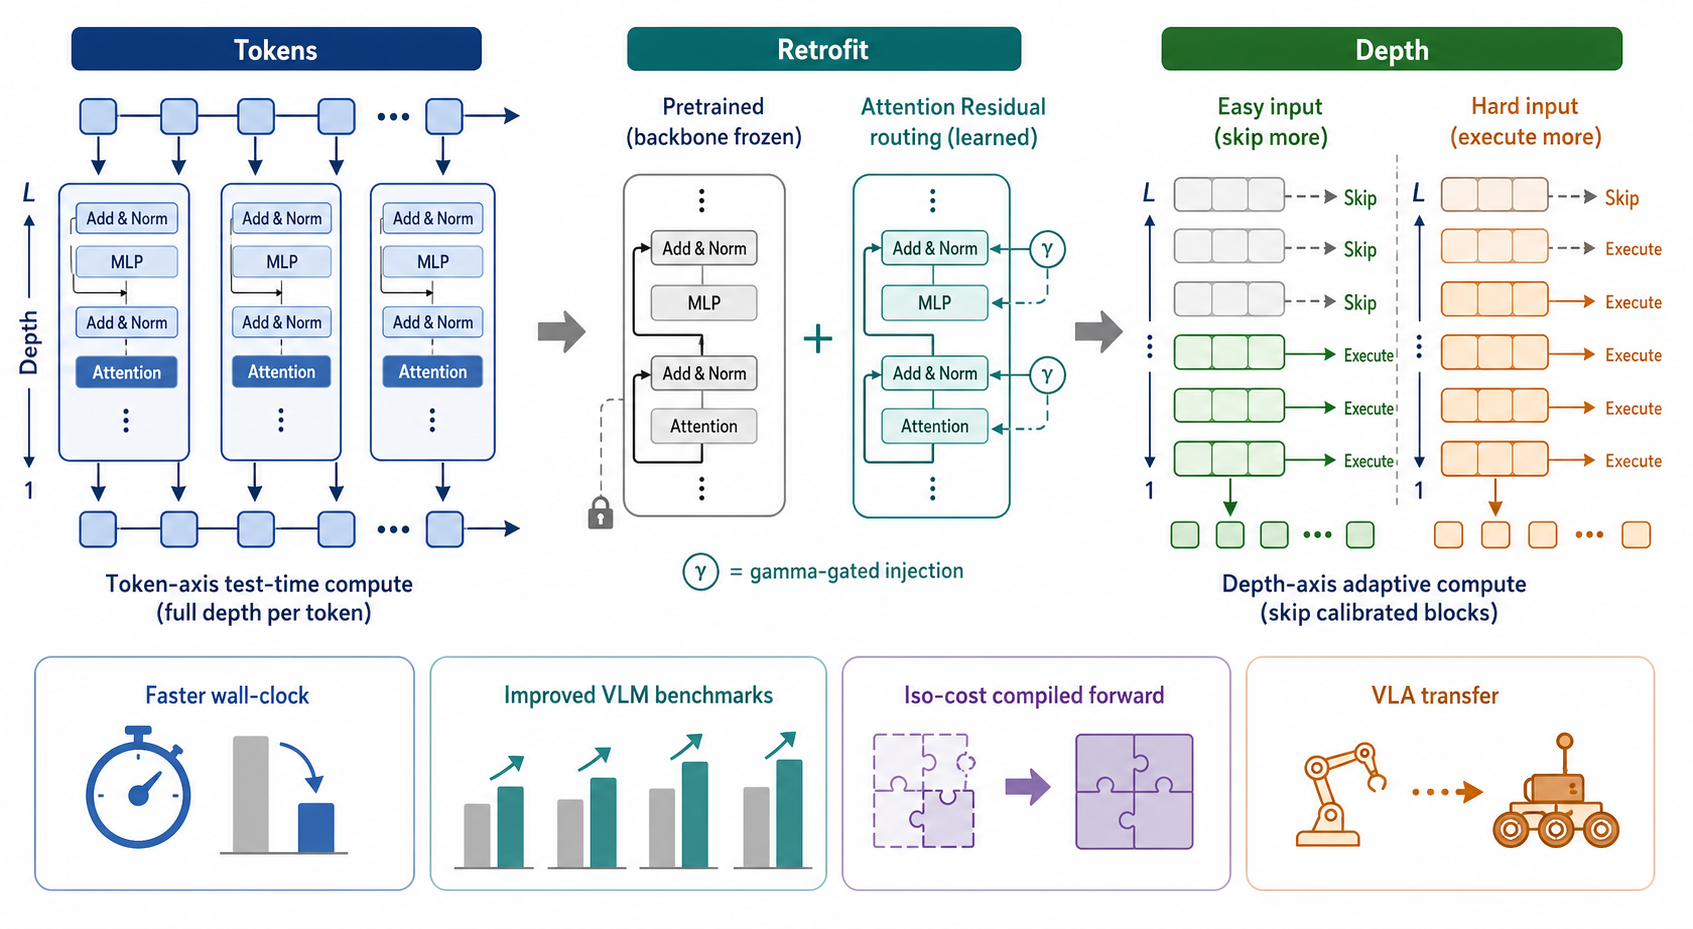
\includegraphics[width=\textwidth]{reskip_main_figure.png}
\caption{\textbf{\retrofit{} 与 \reskip{} 总览。}
\retrofit{} 在一个冻结的预训练骨干上插入 $\gamma$-门控的 \attnres{} 路由，使前向过程作为副产物发出一个预执行的深度信号。\reskip{} 把该信号校准成与输入相关的块执行：容易的输入跳过安全块，困难的输入保留更多深度。retrofit 是主贡献；\reskip{} 是基于已安装路由的自然应用。}
\label{fig:overview}
\end{figure}


%----------------------------------------------------------------------
\section{方法}
\label{sec:method}
%----------------------------------------------------------------------

\subsection{背景：注意力残差}
\label{sec:background}

标准 Transformer 使用固定标量-$1$ 的残差组合 $\mathbf{x}_n = \mathbf{x}_{n-1} + f_n(\mathbf{x}_{n-1})$，不发出任何路由信号。\attnres{}~\citep{chen2026attnres} 把它替换成一个跨深度的可学注意力。每个块 $n$ 维护一个伪查询 $\mathbf{w}_n \in \R^d$；键是先前块输出 $\mathbf{h}_i$ 的投影 $\mathbf{k}_i = W_K \mathbf{h}_i$，并且
\begin{equation}
  \alpha_{i \to n} = \frac{\exp(\mathbf{w}_n^\top \mathbf{k}_i / \sqrt{d})}{\sum_{j=0}^{n-1} \exp(\mathbf{w}_n^\top \mathbf{k}_j / \sqrt{d})},
  \qquad
  \mathbf{x}_n = \sum_{i=0}^{n-1} \alpha_{i \to n}\,\mathbf{h}_i .
  \label{eq:attnres}
\end{equation}
关键性质是\emph{两阶段执行}。计算块 $n$ 的输入只需要 $\{\mathbf{h}_i\}_{i<n}$ 和 $\mathbf{w}_n$——两者都在 $f_n$ 运行\emph{之前}就已就绪。我们把这一预执行注意力计算称为\emph{阶段~1}，把 $f_n$ 本身称为\emph{阶段~2}。阶段~1 就是我们利用的路由信号。块级 \attnres{} 把若干层分组为 $N$ 个块，并在块层级应用 softmax（贯穿全文使用的粒度）。算法~\ref{alg:two_phase}（附录~\ref{app:algorithm}）给出了把 \reskip{} 跳过检查嵌入其中的完整两阶段前向。

\subsection{\reskip{}: \attnres{} 引导的层跳过}
\label{sec:reskip}

\reskip{} 把阶段-1 信号变成一条与输入相关的跳过规则。每个块 $n$ 有两个离线分数：\emph{\attnres{} 重要性} $I(n) = \max_{l > n}\,\E[\alpha_{n \to l}]$（块 $n$ 被多频繁地引用；只需前向）和\emph{消融影响} $A(n) = \mathrm{PPL}(\text{$n$ 被移除}) / \mathrm{PPL}(\text{完整})$（块 $n$ 是否不可替代；$N{-}2$ 次消融前向）。在推理时，对每个 $n$ 我们读取其路由器对前一个块的均权重 $w_{\text{recent}}(n)$，并按下式判断：
\begin{equation}
  \text{跳过块 $n$} \iff
  w_{\text{recent}}(n) > \tau_n
  \;\text{且}\;
  n \in \mathcal{P}
  \;\text{且}\;
  \textstyle\sum_{m<n} \mathbb{1}[\text{已跳过}_m] < M_{\max} ,
  \label{eq:skip_rule}
\end{equation}
其中 $\tau_n$ 按位置校准，取 $32$ 条留出长上下文序列上 $w_{\text{recent}}(n)$ 的第 $q$ 经验分位数（默认 $q{=}0.85$）。判断必须在执行 $\mathrm{Block}_n$ \emph{之前}就拿得到，因此规则只读取来自先前块输出的路由量；相反，基于置信度的早退信号或基于块后隐状态的诊断都做不到这点——它们想跳过当前块就必须先付出运行它的代价（参见附录~\ref{app:method_comparison} 中的 CALM / MoD / pruning / LayerSkip 比较）。\attnres{} 的两阶段前向天然暴露了这样一个预执行信号，跳过判断也只是对阶段~1 已计算量的一次标量比较：无辅助网络、无训练期改动、无架构变动。

\paragraph{路由权重必要但不充分。} 阶段-1 权重是一个有用的跳过\emph{候选}信号，不是安全证书。在我们 $340$M 从零训练的 \attnres{}（图~\ref{fig:reskip_routing}）上，块~$2$ 的重要性中等（$I{=}0.52$），但移除它\emph{毁灭性}地导致 PPL 升至 $8.1\times$；而块~$4$ 的消融影响最小，$I$ 反而高于块~$5$。因此 $\mathcal{P}$ 应同时利用两个信号——低 $I$ 让跳过\emph{常被触发}，低 $A$ 让它\emph{安全}。只看其一严格更差：$\{5\}$ 单独（低 $I$）给出 $1.14\times$；$\{3,5\}$ 组合则给出 $1.19\times$，且 PPL 略低于满深度。带离线消融/漂移扫的校准因此是方法的一部分，而不是事后补丁（附录~\ref{app:reskip_position_ablation}）；同样的协议在 VLM 规模上（按块静态移除，附录~\ref{app:block_removal}）和动作流上（按块动作漂移，附录~\ref{app:vla_pareto}）被复用。

\begin{figure}[t]
\centering

\includegraphics[width=0.95\textwidth]{reskip_routing_importance_vs_ablation.pdf}
\caption{\textbf{\attnres{} 路由权重并不能预测消融影响（340M）。} (a)~学到的块级 $\alpha_{n \to l}$。(b)~$I(n)$（蓝色，左轴）与 $A(n)$（橙色，右轴）。\reskip{} 需要两个信号同时使用。}
\label{fig:reskip_routing}
\end{figure}

这条规则首先要检验一个问题：\attnres{} 中究竟有没有一个可用的内在深度信号。在一个 $340$M 块级 \attnres{} Transformer 上（$d{=}1024$，$L{=}24$，$N{=}8$ 块；FineWeb-Edu 100BT~\citep{penedo2024fineweb}；\texttt{lm-eval-harness}~\citep{eval-harness}），\reskip{} 在 $\mathcal{P}{=}\{3,5\}, M_{\max}{=}2, q{=}0.85$ 下达到 \textbf{$1.19\times$ wall-clock 且基准零下降}，覆盖 LAMBADA~\citep{paperno2016lambada}、HellaSwag~\citep{zellers2019hellaswag} 与 ARC-E/C~\citep{clark2018arc}（表~\ref{tab:reskip_benchmark}；Pareto 与延迟曲线见附录~\ref{app:reskip_results}）。每次前向中跳过次数在 $0$--$2$ 之间变化（$48$ 个 batch 的均值为 $0.88$），证实是真正的输入相关行为，而不是固定块移除。在同样 FineWeb-Edu 配方上对 110M 的跨规模复制在 $q{=}0.97, M_{\max}{=}1$ 下复现了零退化模式（附录~\ref{app:phase1}）。

\paragraph{在相同跳过率下：动态 vs.\ 静态。} 固定 \attnres{} 权重、只改运行时决策规则：在校准的 $\sim$$12\%$ 跳过率附近实际触发的输入相关规则，把 LAMBADA 保持在 $0.345$；而同跳过率下的固定位置/随机切换调度则崩溃到 $0.22$--$0.26$。HellaSwag、PIQA、ARC-E、OpenBookQA 上排序一致。MoD 风格的 ``在相同跳过率下随便哪种调度都能拿到免费收益'' 这一指控因此在 $340$M 上被否定：调度选择本身有意义，且 \attnres{} 路由权重承担了关键作用（完整表格与阈值迁移注意点见附录~\ref{app:b1b2_decision_rule}）。\emph{这验证了在 \attnres{} 内置训练时机制是有效的；更难的问题——如何在已训好的模型中获得它——是 \S\ref{sec:retrofit} 的内容。}

\begin{table}[t]
\caption{\textbf{$340$M 从零 \attnres{} 上的 \reskip{}。} vanilla 行是不带 \attnres{} 的基线（同 FineWeb-Edu 100BT 配方与 tokenizer）。\attnres{}-full 在 7 项任务中提升了其中 6 项相对 vanilla 的表现，且 \reskip{} 在 $q{=}0.85$ 下与之逐位匹配，因为校准的阈值在 lm-eval 分布上几乎不触发（表~\ref{tab:b1b2_observed_rate}）；序列长度 $8192$ 下 $1.19\times$ 的 wall-clock 加速对应零基准下降。表头：PIQA/HellaSwag/ARC-E/ARC-C/OpenBookQA 取 \texttt{acc\_norm}，MMLU/LAMBADA 取常规 \texttt{acc}。$q{=}0.95$ 一行的破折号项在扩展任务集上未重新评估；考虑到观察到的触发率为 $0\%$，预计该行将保持逐位一致。}
\label{tab:reskip_benchmark}
\centering\small
\setlength{\tabcolsep}{3.5pt}
\begin{tabular}{lcccccccc}
\toprule
Configuration & LAMBADA acc & LAMBADA ppl & HellaSwag & PIQA & ARC-E & ARC-C & MMLU & OpenBookQA \\
\midrule
Vanilla (no \attnres{})                    & 0.3790 & 24.71 & 0.4436 & 0.6779 & \textbf{0.5602} & \textbf{0.3046} & \textbf{0.2594} & 0.3320 \\
\midrule
\attnres{} full-depth                       & 0.4054 & 20.20 & 0.4607 & 0.6893 & 0.5438 & 0.3012 & 0.2555 & 0.3580 \\
$+$ \reskip{} ($\{5\}, M{=}1, q{=}0.95$)    & \textbf{0.4054} & \textbf{20.20} & \textbf{0.4607} & --- & \textbf{0.5438} & \textbf{0.3012} & --- & --- \\
$+$ \reskip{} ($\{3,5\}, M{=}2, q{=}0.85$)  & \textbf{0.4054} & \textbf{20.20} & \textbf{0.4607} & \textbf{0.6893} & \textbf{0.5438} & \textbf{0.3012} & \textbf{0.2555} & \textbf{0.3580} \\
\bottomrule
\end{tabular}
\end{table}

\subsection{\retrofit{}: 把 AttnRes 装进一个预训练 Transformer}
\label{sec:retrofit}

retrofit 的目标受引言中的问题约束：拿一个在标准残差体制下预训练的 Transformer，产生一个支持 \attnres{} 的模型，要满足 (P1) 保留基准质量、(P2) 发出足以驱动 \reskip{} 的路由 $\alpha$、(P3) 在已有 SFT 数据上一次较短的微调内训完成且基础模型冻结。要满足第一个约束，修改在第 $0$ 步必须严格保持恒等；要满足第二个约束，路由必须\emph{进入}真实前向路径，而不仅仅是观察它。

我们把 $L$ 个解码器层组织成 $N$ 个 \emph{块}，每块 $L/N$ 层（Qwen3-VL-2B：$L{=}28, N{=}14$）。对每个 $n\ge 1$ 的块，新增一个 \attnres{} 路由器 $\mathbf{w}_n$、一个小适配器 $A_n$（秩-$r$ 的下采样-上采样瓶颈，SiLU）以及一个标量门 $\gamma_n$：
\begin{equation}
  r_n = \sum_{i=0}^{n-1} \alpha_{i \to n}\,h_i, \qquad
  x_n = h_{n-1} + \gamma_n\,A_n(r_n - h_{n-1}), \qquad
  h_n = \mathrm{Block}_n(x_n).
  \label{eq:gamma_gate}
\end{equation}
$\mathrm{Block}_n$ 是预训练块，原封不动；\attnres{} 进入是\emph{在块之间}，作为一个修正项。标准 $r{=}256, L{=}4$ 配置下，retrofit 参数 $\{\mathbf{w}_n, \gamma_n, A_n\}$ 在 2B 上约 $7.4$M（$<0.4\%$），在 4B 上约 $11.8$M（$<0.3\%$）；整个基础模型——嵌入、视觉塔、解码器层、LM 头——都被冻结。

当 $\gamma_n{=}0$ 时，$x_n = h_{n-1}$ 严格成立，因此第 $0$ 步的前向逐位等价于预训练模型。适配器的上投影采用小随机初始化（$\mathcal{N}(0,0.02^2)$），使得在初始处 $\partial\mathcal{L}/\partial\gamma_n \ne 0$，避免梯度死锁。然后我们用线性课程把 $\gamma_n$ 从 $0$ 升到 $1$，跨越前 $30$--$50\%$ 的训练步；每个块都收敛到 $\gamma_n{=}1$，使 retrofit \emph{结构上是纯 \attnres{}}（每个块消费的是路由后的加权和而非标准残差）。我们最初尝试的三种看起来更干净的方案——只观察的头、块输入处的 $\beta\to 1$ 插值、带温度退火的 informed-init 伪查询——都失败了（附录~\ref{app:route_ablations}）。

\reskip{} 重用同一路径，而不是引入新机制。它的阶段-1 决策读取已经计算好的 $\alpha$，当规则触发时短路该块：$h_n\!\leftarrow\!x_n$。为兼容 \texttt{use\_cache=True}，被跳过的块仍要运行其每层产生 K/V 的那一段（\texttt{LayerNorm}\!$\to$\!\texttt{k/v\_proj}\!$\to$\!\texttt{RoPE}\!$\to$\!\texttt{cache.update}），其代价约为完整层前向的 $5$--$10\%$，但跳过 \texttt{q\_proj} / 注意力 / \texttt{o\_proj} / MLP。组合后的 \texttt{skip\,+\,use\_cache=True} 路径与无 cache 路径在末位 argmax 上一致（附录~\ref{app:kv_equiv}）。

训练目标由上述三个约束直接给出。我们最小化
\begin{equation}
  \mathcal{L} = \mathcal{L}_{\text{CE}}(\text{完整路径}) + \lambda_{\text{kl}}\,\mathcal{L}_{\text{KL}}(\text{跳过路径}\,\|\,\text{teacher}) + \lambda_{\text{ent}}\,\mathcal{L}_{\text{ent}}(\alpha) ,
  \label{eq:retrofit_loss}
\end{equation}
其中 $\mathcal{L}_{\text{CE}}$ 在助手 token 上计算；跳过分支的 KL 每步随机采样一个块跳过，运行该跳过下的前向，并把得到的 logits 拉向一个冻结的预训练教师（这样代理 $x_n$ 在块运行时和被跳过时都有用）。$\mathcal{L}_{\text{ent}}$ 在损失中带负号，即一个轻度的最大熵先验，防止 $\alpha$ 早期过早坍缩。默认 $\lambda_{\text{kl}}{=}1$、熵权 $0.02$、retrofit 参数学习率 $10^{-3}$、$100$ 步 warmup 的余弦调度。超参数与全文使用的 v1 / v3 数据混合在附录~\ref{app:retrofit_hparams} 列出。

这不是普通的 SFT。CE 项让完整路径对下游任务保持有用，但它本身并不训练跳过代理去替代一个真实块。跳过分支的 KL 通过把每步一次跳过-块前向绑定到冻结教师来提供这一约束。反过来，纯教师模仿只会复现基础模型。弱熵先验防止早期单源坍缩，同时仍允许路由器在后期变锐。这种三项结构正是让 retrofit 在第 $0$ 步保持恒等、在训练后改进任务、在推理时具备跳过能力的关键。

%----------------------------------------------------------------------
\section{实验：在 Qwen3-VL-2B 与 4B 上的 \retrofit{}}
\label{sec:experiments}
\label{sec:exp_retrofit}
%----------------------------------------------------------------------

第一个实证问题是：retrofit 是否在不简单牺牲预训练模型能力的前提下解决了安装问题。我们在 $L{=}4$、$N{=}7$ 的块划分上对 \textbf{Qwen3-VL-2B}~\citep{bai2025qwen3vl}（$L{=}28, d{=}2048$）做 retrofit，并在 $L{=}4$、$N{=}9$ 的块划分上对 \textbf{Qwen3-VL-4B}（$L{=}36, d{=}2560$）做 retrofit（块划分扫见附录~\ref{app:block_partition}）。所有基础参数都被冻结；在 $r{=}256$ 下，$2$B 的 retrofit 参数约 $7.4$M、$4$B 约 $11.8$M，按 Eq.~\ref{eq:retrofit_loss} 训练。标准 SFT 混合为 $60\%$ LLaVA-OneVision-Data~\citep{li2024llavaonevision} + $20\%$ UltraChat + $10\%$ NuminaMath + $10\%$ OpenThoughts，训练 $10$k 步。评估使用 LAMBADA~\citep{paperno2016lambada}/HellaSwag~\citep{zellers2019hellaswag} 评估文本，使用六个 \texttt{lmms-eval} 基准评估 VLM（MMBench~\citep{liu2023mmbench}、MMMU~\citep{yue2024mmmu}、MMStar~\citep{chen2024mmstar}、AI2D~\citep{kembhavi2016ai2d}、OCRBench~\citep{liu2024ocrbench}、RealWorldQA~\citep{grok2024realworldqa}）。

\begin{table}[t]
\caption{\textbf{Qwen3-VL-2B/4B 上标准 $L{=}4$ v3 配方下的 \retrofit{}}（VLM 用 \texttt{lmms-eval} 全集，LAMBADA/HellaSwag 用 $n{=}2000$）。retrofit 在两种规模上都严格改进了 $5/6$ 个 VLM 基准，并在文本侧提升 LAMBADA（$2$B 上 $+3.3$pp；$4$B 上 $+8.7$pp）。MMStar 总体持平；其 math 子类（附录~\ref{app:mmstar_subcat}）跃升 $2$B 上 $+7.9$pp / $4$B 上 $+3.9$pp——为整套基准中最大的单格变化，和路由器倾向于提升深思推理路径的解释一致（\S\ref{sec:exp_retrofit}）。参数匹配的 LoRA 基线无法复现文本增益（4 次平均 LAMBADA $-0.6$pp；附录~\ref{app:lora_baselines}）。本表所有准确率结果都在标准 $L{=}4$ retrofit 前向（无跳过）下评估，作为 \S\ref{sec:exp_retrofit} 中 wall-clock 参考。}
\label{tab:retrofit_main}
\centering\small
\setlength{\tabcolsep}{4pt}
\begin{tabular}{lcccccccc}
\toprule
& \multicolumn{2}{c}{Text} & \multicolumn{6}{c}{VLM (\texttt{lmms-eval} full split)} \\
\cmidrule(lr){2-3}\cmidrule(lr){4-9}
Configuration & Lamb. & HSwag & MMB & MMMU & MMStar & AI2D & OCR & RWQA \\
\midrule
Qwen3-VL-2B Base (LoRA)               & 53.2 & 50.6 & 75.8 & 41.4 & 53.6 & 73.6 & 77.2 & 64.8 \\
$+$ \retrofit{}                       & \textbf{56.5} & 50.0 & \textbf{78.9} & \textbf{43.2} & 53.6 & \textbf{75.8} & \textbf{81.4} & \textbf{66.1} \\
~~~~$\Delta$ vs.\ base                & \textbf{+3.3} & $-0.6$ & \textbf{+3.1} & \textbf{+1.8} & $0.0$ & \textbf{+2.2} & \textbf{+4.2} & \textbf{+1.3} \\
$+$ \reskip{}                         & 56.1 & 49.2 & 78.9 & 43.0 & \textbf{54.9} & \textbf{75.9} & 80.1 & 66.0 \\
\midrule
Qwen3-VL-4B Base (LoRA)               & 57.6 & 56.2 & 83.3 & 49.0 & 62.4 & 81.9 & 81.9 & 71.5 \\
$+$ \retrofit{}                       & \textbf{66.3} & 55.2 & \textbf{85.2} & \textbf{52.1} & \textbf{63.2} & \textbf{82.5} & \textbf{82.4} & \textbf{71.8} \\
~~~~$\Delta$ vs.\ base                & \textbf{+8.7} & $-1.0$ & \textbf{+1.9} & \textbf{+3.1} & \textbf{+0.8} & \textbf{+0.6} & \textbf{+0.5} & \textbf{+0.3} \\
$+$ \reskip{}                         & 63.3 & 54.9 & 85.0 & 51.4 & 62.1 & 82.5 & 82.5 & 70.7 \\
\bottomrule
\end{tabular}
\end{table}


标准 retrofit 给出了对第一个问题的肯定回答（表~\ref{tab:retrofit_main}）：在 $2$B 上严格高于基线于六个 VLM 基准中的五个（第六个 MMStar 在总和上保持在 $\pm 0$pp 内），在 $4$B 上六个基准全部高于基线。最大的单格变动出现在 MMStar 的 math 子类（$2$B 上 $+7.9$pp、$4$B 上 $+3.9$pp）；在 $2$B 上这一增益在 MMStar 内部被 sci\&tech 的 $-5.5$pp 与 instance-reasoning 的 $-2.7$pp 抵消（六格完整分解见附录~\ref{app:mmstar_subcat}），因此路由器看起来是在选择性地把权重重新分配到逐步推理路径，而不是在均匀地拉升推理能力。文本质量也提升：$2$B 上 $+3.3$pp LAMBADA / $-16\%$ ppl，$4$B 上 $+8.7$pp / $-32\%$（$4$B 上的跳跃在 $L{=}2$ 与 $L{=}4$ 块划分上都复现，附录~\ref{app:block_partition}）；HellaSwag 在两种规模上都在 $\pm 1.1$pp 之内。每个块都收敛到 $\gamma_n{=}1$，因此 retrofit 在结构上是纯 \attnres{}。

第二个问题是归因：这些增益是由 \attnres{} 路径带来的，还是仅仅因为加了一个小可训模块。表~\ref{tab:attribution} 在相同数据与步数预算下把 \retrofit{} 与三种参数匹配的替代方案在 Qwen3-VL-$2$B 上做了比较。在 $\{q,k,v,o\}$ 或 MLP 上的参数匹配 \textbf{LoRA} 在 4 次运行中的 LAMBADA 平均为 $0.526$（比基线低 $0.6$pp），排除 ``增益只是来自 $15$M 可训参数'' 的解释。\textbf{Observer-only} 路由学一个不反馈到前向的 $\alpha$ 头；LAMBADA 崩塌到 $0.12$，表明路由必须是承载信号的而不是被动副信号。\textbf{$\gamma$-free} 变体（$\gamma_n{\equiv}0$ 在零附近可训，适配器主导）是一个强适配器基线：它复原了 LAMBADA 增益，并在 MMBench 上与 canonical 持平。但它的残差路径仍是 $h_{n-1} + \mathrm{adapter}(\cdot)$，因此模型在结构上从未变成 \attnres{}，其 $\alpha$ 是副产物而不是 \reskip{} 或动作流跳过可读取的真实深度分配信号。只有 $\gamma{\to}1$ 的 canonical 配方最终把残差路径改写成路由后的加权和。

\begin{table}[t]
\caption{\textbf{归因：在 Qwen3-VL-$2$B 上 \retrofit{} vs.\ 参数匹配的替代方案。} 同样的训练混合与步数预算。``Structural \attnres{}'' 表示训练后模型的残差路径 $x_n$ 是否等于路由加权和 $\sum_i \alpha_{i\to n}\,h_i$（\emph{yes}），还是仍是 $h_{n-1}+\mathrm{adapter}(\cdot)$（\emph{no}）。只有 \textbf{Structural=yes} 一行能支撑 \reskip{} 的阶段-$1$ 深度信号。}
\label{tab:attribution}
\centering\small
\begin{tabular}{lccccc}
\toprule
Method & New params & Structural \attnres{} & LAMBADA & HellaSwag & MMBench \\
\midrule
Qwen3-VL-$2$B (base)                       & ---         & ---     & $0.532$ & $0.506$ & $75.77$ \\
LoRA (mean of $4$)                         & $\sim$$15$M & no      & $0.526$ & $0.509$ & --- \\
Observer-only                              & $\sim$$15$M & signal only & $0.12$  & ---     & --- \\
$\gamma$-free (adapter, $\gamma{\approx}0$)& matched & no      & $0.576$ & $0.512$ & $0.720$ \\
\textbf{\retrofit{} ($\gamma{\to}1$, ours)}& $\sim$$7.4$M & \textbf{yes} & $\mathbf{0.576}$ & $\mathbf{0.522}$ & $\mathbf{0.710}$ \\
\bottomrule
\end{tabular}
\end{table}

第三个问题是：装好的信号是否可用于深度分配。在按规模选取的可跳块集合（$2$B：$\mathcal{P}{=}\{1,4\}$；$4$B：$\mathcal{P}{=}\{1,2\}$）和按块校准的阈值下，动态跳过在保守端保持质量（见主表与附录~\ref{app:retrofit_pareto}）。同样的 Pareto 形状在动作预测上重新出现（\S\ref{sec:vla}），验证了同一阈值校准协议下深度轴分配从 token 级到动作级解码的迁移性。

最后，retrofit 的前向路径必须在部署期保持实用。在保守工作点下启用动态 \reskip{}，retrofit 的 wall-clock 与基础模型在 H100/bf16、序列长度 $2048$ 上持平（表~\ref{tab:retrofit_latency}；compile / eager / skip 配置完整分解见附录~\ref{app:latency}）。\S\ref{sec:reskip} 中 $340$M 从零 \attnres{} 在同一 \reskip{} 规则下处于 $1.19\times$ wall-clock，因此该路由信号同时支持两种范式。

\begin{table}[t]
\caption{\textbf{标准工作点下的前向 wall-clock}，$1{\times}$H100、bf16、batch~$1$、seq~$2048$，$5$ 次预热后 $20$ 次的中位数。retrofit 行使用 $q{=}0.99$、$\mathcal{P}{=}\{1,4\}$、$M_{\max}{=}2$ 的动态 \reskip{}。完整分解（eager / compile 模式、划分扫、VLA 在骨干内的对照）见附录~\ref{app:latency}。}
\label{tab:retrofit_latency}
\centering\small
\setlength{\tabcolsep}{4pt}
\begin{tabular}{lcc}
\toprule
Configuration & ms & vs.\ base \\
\midrule
Qwen3-VL-2B (base)                          & $25.49$ & --- \\
$+$ \retrofit{} $+$ \reskip{}               & $\sim 26.0$ & $\approx 1.02\times$ \\
\bottomrule
\end{tabular}
\end{table}

%----------------------------------------------------------------------
\section{VLA 应用}
\label{sec:vla}
%----------------------------------------------------------------------

VLA 测试用来分离两件事：retrofit 是否能\emph{迁移}到下游控制任务上，以及它的热启动是否可以被 ``直接在 VLA 数据上跑 $\gamma$-课程'' 替代。视觉 token（感知，浅层~\citep{raghu2021vision}）、语言 token（任务描述）、动作 token（运动规划）没有原则性的理由共享相同的有效深度；\attnres{} 路由给出了一个按位置可控的把手，无需任何 token 级门控机制。

我们把 OpenVLA-OFT~\citep{kim2025openvlaoft} 动作头（$L_1$ 回归，无分块）接到 Qwen3-VL-2B/4B 骨干（ViT 冻结）上，并在 LIBERO~\citep{liu2023libero} 的合并 \texttt{libero\_all} 混合上训练。实验围绕两个问题：VLM retrofit 是否对控制是有用的热启动，以及同样的架构是否能仅靠 VLA 数据学习追上来。三条路径共享头与数据：\textbf{Path 0}（原始骨干 OFT，基线）、\textbf{Path B}（从我们标准的 $L{=}4$ v3 $10$k VLM retrofit 热启动，$\gamma_n{=}1$ 全程）、\textbf{Path C}（与 Path B 同架构但\emph{无 VLM retrofit}；路由器/适配器随机初始化，$\gamma$ 在 VLA 数据上从 $0$ 升到 $1$）。$4{\times}$H100 ZeRO-2，有效 batch $32$，$30$k 步。每个策略每个套件 $500$ 次 rollout（每策略共 $2{,}000$）。两个 $2$B 重复 rollout 单元的种子细节见附录~\ref{app:vla_variance}；$4$B 上一个 instruction-action 词表陷阱（旧的混淆来源；现已通过 clean base 解决）见附录~\ref{app:vla_pitfall}。

\subsection{LIBERO 结果}
\label{sec:vla_results}

\begin{table}[t]
\caption{\textbf{Qwen3-VL-2B/4B 在三条训练路径下的 LIBERO 4 套件成功率（\%）}。条目是每套件 $500$ 次 rollout（每策略 $2{,}000$）的成功率。\emph{Path 0} 是原骨干 OFT 基线；\emph{Path B} 从我们标准的 $L{=}4$ v3 $10$k VLM retrofit 热启动；\emph{Path C} 跳过 VLM retrofit，直接在 VLA 数据上跑 $\gamma$-课程。Clean 4B 表示不向基础 VLM 添加 action-token 嵌入（附录~\ref{app:vla_pitfall}）。Path B 是两种规模下推荐的热启动配置。$2$B 的 \texttt{Goal} 与 \texttt{Long-10} 单元是两次 rollout 的按种子均值（附录~\ref{app:vla_variance}）；其他单元在两种规模下都是单次 rollout。}
\label{tab:vla_libero}
\centering\small
\setlength{\tabcolsep}{4pt}
\begin{tabular}{llcccccc}
\toprule
Scale & Policy & Spatial & Object & Goal & Long-$10$ & \textbf{Avg} & $\Delta$ vs.\ Base \\
\midrule
2B & Base               & $94.8$ & $99.8$ & $97.4$ & $91.4$ & $95.9$ & --- \\
2B & Full               & $\mathbf{97.8}$ & $99.6$ & $98.6$ & $92.6$ & $97.2$ & $\mathbf{+1.3}$ \\
2B & \reskip{}          & $97.6$ & $99.2$ & $\mathbf{99.0}$ & $\mathbf{93.6}$ & $\mathbf{97.4}$ & $\mathbf{+1.5}$ \\
\midrule
4B & Base               & $95.0$ & $99.2$ & $97.8$ & $92.2$ & $96.1$ & --- \\
4B & Full               & $94.6$ & $\mathbf{99.8}$ & $98.2$ & $\mathbf{94.2}$ & $\mathbf{96.7}$ & $\mathbf{+0.7}$ \\
4B & \reskip{}          & $\mathbf{96.4}$ & $98.2$ & $\mathbf{98.4}$ & $92.8$ & $96.5$ & $+0.4$ \\
\bottomrule
\end{tabular}
\end{table}

Full AR-Retrofit 在两种规模上都肯定地回答了热启动问题：$2$B 上 $97.2\%$，干净 $4$B 基础上 $96.7\%$，在四套件聚合上分别比 matched Base 改进 $+1.3$pp / $+0.7$pp。我们的解读不是 \retrofit{} 解决了 VLA，而是：经过 retrofit 的深度路由骨干能在不损害控制的前提下迁移过来，并在那些依赖骨干质量的套件上提供有利的热启动。

Path C 否定了替代问题。它在 $30$k 同预算下停在 $94.30\%$，落后 Path B $2.45$pp。差距最大的是 Spatial（Path C $92.6$ vs.\ Path B $97.8$，$5.2$pp），那也是稳定的预训练路由器最关键的位置：仅在 \texttt{libero\_spatial} 任务~$6$ 上，Path C 是 $50\%$、Path B 是 $78\%$。因此 VLM retrofit 起的是高层骨干的有用初始化作用，不是一个 VLA-only 训练能复现的可替代热启动。

\subsection{\reskip{} 在动作流上}
\label{sec:vla_reskip}

我们现在把同一条 \reskip{} 规则在推理时应用到训练好的 Path B 策略上，但阈值在仿真 rollout 分布上校准而不是语言 token（理由在下一段）。可跳块按规模从按块动作漂移扫选取（附录~\ref{app:vla_pareto}：$2$B 上 $\mathcal{P}{=}\{1,4\}$、$4$B 上 $\mathcal{P}{=}\{1,2\}$），$M_{\max}{=}2$ 全程不变。表~\ref{tab:vla_reskip_pareto} 给出 4 套件 Pareto 随 $q$ 的变化。

\begin{table}[t]
\caption{\textbf{训练好的策略上的 \reskip{} 4 套件 Pareto}。可跳块 $\mathcal{P}$ 与阈值 $\tau$ 按规模在动作分布上校准；$q$ 是产生 $\tau$ 的经验分位。无跳过参考对应主表 Full policy：2B 为 $97.2$，4B 为 $96.7$。保守端（这里 $q{=}0.99$）是推荐工作点：2B 为 $97.4$，4B 为 $96.5$。}
\label{tab:vla_reskip_pareto}
\centering\small
\setlength{\tabcolsep}{4pt}
\begin{tabular}{lccccc}
\toprule
$q$ (sim-calibrated) & Spatial & Object & Goal & Long-$10$ & \textbf{Avg} \\
\midrule
\multicolumn{6}{l}{\emph{Qwen3-VL-2B, $\mathcal{P}{=}\{1,4\}, M{=}2$, no-skip/full ref $97.2$}} \\
\midrule
$0.30$              & $4.7$  & ---     & ---     & ---     & (collapse) \\
$0.85$              & $80.0$ & $98.0$  & $87.3^\ast$ & $67.2$  & $83.1$ \\
$0.95$              & $95.0$ & $99.4$  & $97.6$  & $86.8$  & $94.7$ \\
$\mathbf{0.99}$     & $\mathbf{97.6}$ & $\mathbf{99.2}$  & $\mathbf{99.0}$  & $\mathbf{93.6}$  & $\mathbf{97.4}$ \\
no-skip/full (ref)  & $97.8$ & $99.6$  & $98.6$  & $92.6$  & $97.2$ \\
\midrule
\multicolumn{6}{l}{\emph{Qwen3-VL-4B, $\mathcal{P}{=}\{1,2\}, M{=}2$, no-skip/full ref $96.7$}} \\
\midrule
$0.30$              & $89.6$ & $95.4$  & $96.4$  & $86.0$  & $91.85$ \\
$0.50$              & $91.2$ & $98.0$  & $98.2$  & $89.6$  & $94.25$ \\
$0.85$              & $93.6$ & $99.2$  & $97.6$  & $93.2$  & $95.90$ \\
$0.95$              & $95.6$ & $98.0$  & $98.0$  & $93.0$  & $96.15$ \\
$\mathbf{0.99}$     & $\mathbf{96.4}$ & $\mathbf{98.2}$  & $\mathbf{98.4}$  & $\mathbf{92.8}$  & $\mathbf{96.5}$ \\
no-skip/full (ref)  & $94.6$ & $99.8$  & $98.2$  & $94.2$  & $96.7$ \\
\bottomrule
\multicolumn{6}{p{14cm}}{\footnotesize $^\ast$部分评估（$332/500$ 次试验）——驱动器调度被截断；按已完成试验的成功率报告。}
\end{tabular}
\end{table}

阈值在动作分布上校准而不是从语言迁移：把 LAMBADA 校准、$q{=}0.85$ 的阈值幼稚地用到同一策略上会让 LIBERO-Spatial 崩塌到 $64\%$（附录~\ref{app:vla_pareto}）。原因是 $q$ 本身不是跳过率；它给出的是 $w_{\text{recent}}$ 的一个尖锐经验分布的索引。VLA 推荐工作点因此偏保守（$q{=}0.99$）：跳得很少，且仅在按块动作漂移扫认定为局部安全的块上跳。按规模选 $\mathcal{P}$ 的按块动作漂移扫、跨模态阈值迁移失败、按种子分解、流水线陷阱、以及一份开源 VLA 在 LIBERO 上的对照表（$\pi_0$ / OpenVLA / SpatialVLA）见附录~\ref{app:vla_variance},\,\ref{app:vla_pitfall},\,\ref{app:vla_landscape},\,\ref{app:vla_pareto}。

%----------------------------------------------------------------------
\section{相关工作}
\label{sec:related}
%----------------------------------------------------------------------

在测试期算力方面，o1~\citep{openai2024o1}、DeepSeek-R1~\citep{deepseek2025r1}、思维链~\citep{wei2022chain} 以及最优测试期算力分析~\citep{snell2024scaling} 都是通过发出更多推理 \emph{token} 来分配算力；每 token 的深度仍然固定。深度轴方法包括 ACT / Universal Transformer~\citep{graves2016adaptive, dehghani2018universal}、CALM~\citep{schuster2022confident}、Mixture-of-Depths~\citep{raposo2024mixture}、LayerSkip~\citep{elhoushi2024layerskip} 与静态裁剪~\citep{gromov2024unreasonable, men2024shortgpt}。它们各自加了停机头、退出分类器、路由器、推测解码器或静态删除规则。我们则使用 \attnres{} 作为前向计算自身产生的内在路由信号，并把这个信号通过 retrofit 安装进现有的预训练骨干。

神经层面的动机是把循环作为弹性有效深度。双过程理论~\citep{kahneman2011thinking} 自然映射到视觉处理：容易的刺激可由前馈通路处理，更难的刺激则会调动循环回路~\citep{lamme2000distinct, kar2019recurrent, dicarlo2012does}。循环网络能刻画人类的表征动力学~\citep{kietzmann2019recurrence}；\citet{spoerer2020recurrent} 是最接近的概念前驱，他们指出循环 CNN 可以在更难的图像上花更多步以解释速度--准确率行为。循环也有一种深度解释：有限循环可以展开成前馈深度，但循环形式重用一个固定衬底以提供弹性有效深度~\citep{vanbergen2020going}。我们把这点当作设计目标，而不是认知忠实性主张：皮层微回路与树突联合~\citep{bastos2012canonical, buschman2007topdown, larkum2013cellular} 启发我们做内在路由，而我们的实现仍是一个 Transformer retrofit。

在残差架构方面，DenseNet~\citep{huang2017densely} 与 Highway 网络~\citep{srivastava2015highway} 修改了残差流；\attnres{}~\citep{chen2026attnres} 用深度注意力推广了残差组合。我们是第一个把这些权重作为跳过信号暴露出来、也是第一个把它们装入预训练 Transformer 的工作。在 VLA 方面，RT-2~\citep{brohan2023rt}、Octo~\citep{team2024octo}、OpenVLA~\citep{kim2024openvla} 与 Pi0~\citep{black2024pi0} 奠定了范式；效率工作主要集中在动作分块~\citep{zhao2023learning} 与事后压缩。我们贡献的是 VLM 骨干侧的、模态感知的自适应深度。

\section{讨论}
\label{sec:discussion}
%----------------------------------------------------------------------

\retrofit{} 通过一次较短的微调把一种内在的深度路由信号装进一个冻结的预训练 Transformer；得到的路由权重作为自然应用驱动 \reskip{}。在标准的 $L{=}4$ v3 配方下，retrofit 在六个 VLM benchmark 上平均提升 $+2.1$pp / $+1.2$pp，并把 LAMBADA 抬高 $+3.3$/$+8.7$pp。装好的信号是可用的：在 $340$M 从零模型上，\reskip{} 保持 AttnRes 分数并恢复大部分新增推理开销，跳过率匹配的对照下输入相关规则严格优于静态/随机调度。从 retrofit 热启动的 LIBERO VLA 相对匹配 OFT 基线提升 $+1.3$pp / $+0.7$pp；动作流上以动作分布重新校准阈值的 \reskip{} 在保守工作点保持训练好的策略。

\paragraph{主张范围。} 本结果应被解读为一个证据：预训练 Transformer 可以通过轻量 retrofit 获得可用的深度路由通路，而不是说所得到的 \reskip{} 策略是普遍最优的、或低 \attnres{} 权重单独足以认证安全的层移除。在所有大模型与 VLA 实验中，可跳块资格都通过按块消融或动作漂移校准，阈值都在被解码模态上校准。\reskip{} 当前是一个 eager 模式算子；将它与 \texttt{torch.compile} 组合需要一个静态图变体的跳过规则，这是开放的系统工作（附录~\ref{app:latency}）。retrofit 在两种规模上仅在一个 VLM 系列上验证；对其他骨干的迁移仍是开放的。

\bibliography{references}

%----------------------------------------------------------------------
\appendix
\section{局限与未来工作}
\label{app:limitations}
%----------------------------------------------------------------------

\paragraph{局限。}
(i)~只有一个 VLM 系列上的两个 retrofit 目标；将其扩展到 InternVL / Gemma-VL / 纯文本 LM 已在计划之中。(ii)~报告的 wall-clock 是 eager 模式下的动态 \reskip{}。一个静态图变体的跳过规则（按形状桶固定路由的 compile-safe top-$k$）将允许 \texttt{torch.compile} 与 \reskip{} 共存并叠加各自的节省；这是开放的系统工作。(iii)~Wall-clock 是 H100 / bf16；中低端 GPU / 边缘端的测量尚未做。(iv)~VLA Pareto 的阈值是按规模在仿真上校准的，不是在单次 rollout 内\emph{按模态}校准；按模态、按 token 类的校准是下一个扫的目标。(v)~块级粒度继承自 \attnres{}；按 token 路由属于未来工作。

\paragraph{未来工作：权重共享 AttnRes（\reloop{}）。}
一个自然的扩展是让块权重在深度上共享，由位置索引的伪查询区分每次应用；\attnres{} 路由权重就同时承担停机信号，把 \reskip{}（``低 $\alpha$ $\Rightarrow$ 跳过块''）与一种 \reloop{} 停机规则（``低均近 $\alpha$ $\Rightarrow$ 停止迭代''）统一起来。一个 74M 验证产生了平滑的深度--质量 Pareto（节省 $25\%$ 算力 $<1\%$ ppl 变化）；扩规模并与 retrofit 框架结合是开放的。

\section{实现细节}
\label{app:implementation}
%----------------------------------------------------------------------

\subsection{带跳过的在线 softmax 合并}
当一个块被跳过时，在线 softmax 合并就不处理它的输出。运行状态 $(\mathbf{s}, m, e)$ 不变。输出在数学上与一个该块未贡献的 \attnres{} 模型等价——前提是后续的 $\mathbf{w}_l$ 校准。

\subsection{伪查询初始化（\S\ref{sec:reskip} 从零训练）}
对于从零训练，我们使用 $\mathbf{w}_l \sim \mathcal{N}(0, 0.02)$，初始时给出近均匀的 $\alpha$，在前几千步内逐渐特化。

\subsection{Retrofit 超参数}
\label{app:retrofit_hparams}
AdamW，$\beta{=}(0.9,0.95)$，weight decay 为 $0$，梯度裁剪 $1.0$，bfloat16。retrofit 参数（路由器、适配器、$\gamma$）的学习率为 $10^{-3}$，余弦调度，$100$ 步 warmup。序列长度 $1536$（训练）/ $2048$（评估）。损失权重 $\lambda_{\text{kl}}{=}1$，熵权 $0.02$，KD 温度 $1$。熵项以负号进入损失，即在训练早期最大化路由熵而不是最小化它。跳过分支采样：每步在合格块中均匀随机抽一个。适配器瓶颈秩 $r{=}256$（标准）；路由器键的位置偏置启用；路由器温度固定为 $1$。$\gamma$-课程：$0\to 1$ 线性，跨越总步数前 $30\%$（$2$B $5$k/$10$k、$4$B $5$k），$4$B $\times 10$k 用 ramp-fraction $0.5$ 以稳定一次后期 $\gamma{=}1$ 转换发散（附录~\ref{app:gamma_stability}）。单卡 H100 上的总训练 wall-clock：$2$B $5$k 约 $22$ 分钟，$2$B $10$k 约 $44$ 分钟，$4$B $10$k 约 $54$ 分钟。

\subsection{块粒度}
\label{app:block_granularity}
最终配方在两种规模上都使用每块 $L{=}4$ 层：Qwen3-VL-2B 共 $N{=}7$ 块、Qwen3-VL-4B 共 $N{=}9$ 块。早期的 $L{=}2$ 仍作为消融与历史对照保留在附录中，但 $L{=}4$ 是标准设定，因为它在保留准确率平台的同时把路由器调用数相对 $L{=}2$ 减半。每块得到一个路由器、一个残差适配器（默认 $r{=}256$）和一个标量 $\gamma$ 门。

\subsection{初始恒等细节}
\label{app:identity}
当 $\gamma_n{=}0$ 且适配器上投影按 $\mathcal{N}(0, 0.02^2)$ 初始化时，retrofit 前向在算术上与预训练模型完全等价（两者都得到 $x_n = h_{n-1}$，并送入未修改的块）。我们端到端验证了这点：在 LAMBADA 的 $n{=}500$ 上，retrofit 与 base 在 bfloat16 评估噪声内一致（acc $0.530$ vs.\ $0.532$；ppl $5.572$ vs.\ $5.547$）；在 MMMU 与 MMStar 上它们在选项级别逐位相等。token 级 smoke test 显示 $|\Delta\text{logits}|$ 最大为 $0.375$（bfloat16 SDPA 噪声），且在我们的校准 prompt 上 argmax $100\%$ 一致。

\subsection{\texorpdfstring{\texttt{use\_cache=True} 下跳过：正确性验证}{Skip under use cache: correctness verification}}
\label{app:kv_equiv}
我们验证 \S\ref{sec:retrofit} 描述的 K/V-only 跳过路径与无 cache 路径产生 argmax 一致的输出。流程：对一个固定 prefill 输入，用相同的跳过配置对 retrofit 跑两遍——一次 \texttt{use\_cache=False}，一次 \texttt{use\_cache=True}——并比较末位 argmax 与 logits。我们在 H\_r256\_5k Qwen3-VL-2B 上扫了跳过集 $\{[4]$、$[4,10]$、$[4,10,12]$、$[2,4,10]\}$。在每一种配置下，两种 cache 模式的末位 argmax 都匹配，最大 logit 差为 $0.19$--$0.37$，与未做 retrofit、不跳过的原 base 上观察到的 bfloat16 SDPA 抖动一致。从位置 $27$--$40$ 起开始的多步自回归发散，是 HF $+$ bf16 $+$ SDPA 在相同 prompt 上（``Once upon a time''、``def fibonacci''）即使在原 base 也表现出来的固有性质，并不是我们跳过路径带来的。

\subsection{\texorpdfstring{$\gamma{=}1$ 转换稳定性}{gamma=1 transition stability}}
\label{app:gamma_stability}
在 v3 混合、$10$k 步、ramp-fraction $0.3$ 下，Qwen3-VL-4B 在大约第 $3{,}125$ 步发散（训练 CE 从 $0.9$ 升到 $6.5+$）。同样配置在 $5$k 步、以及 $10$k 步用 v3-VL-only 混合（同样 ramp-fraction，但推理梯度密度被降低）下都稳定收敛。把 ramp 延长到 $0.5$（ramp 在第 $5{,}000$ 步而不是第 $3{,}000$ 步结束）在 $4$B $\times 10$k 上恢复了收敛，对最终质量没有可测影响：$4$B $\times 10$k 在 ramp $0.5$ 下，每个 VLM 基准都与 $4$B $\times 5$k 在 ramp $0.3$ 下相差 $1$pp 以内，因此 ramp-fraction 的差异不会污染附录~\ref{app:block_partition} 中的单元间对比。工作经验：只要 $\gamma{=}1$ 转换发生在 $\geq 5{,}000$ 步，则在我们测试过的所有规模与划分上都稳定。

%----------------------------------------------------------------------
\section{Retrofit 消融与推理机制}
\label{app:ablations}
%----------------------------------------------------------------------

\subsection{早期被否决的设计}
\label{app:route_ablations}
早期方案尝试了：(i)~observer-only（不改前向；$\alpha$ 由蒸馏训练）；(ii)~块输入处插值 $\beta{=}\sigma(\text{logit})$ 并推向 $1$；(iii)~纯 AttnRes，伪查询用 $\mathbf{w}_n \gets c\,\bar{\mathbf{k}}_{n-1}$ informed-init + 温度退火。(i) 产生的 $\alpha$ 头其跳过决策不会通过前向反馈，导致 LAMBADA 准确率崩到 $0.12$；(ii) 一旦 $\beta$ 增大就把冻结的 backbone 推离分布，需要预训练数据才能恢复（违背 ``轻量微调'' 的前提）；(iii) 对预训练 backbone 中相邻层的 key 相似度高度敏感，且在我们的训练预算内不收敛。$\gamma$-门控残差注入（\S\ref{sec:retrofit}）是收敛的配方。

\subsection{适配器秩消融}
\label{app:rank_ablation}
不同秩之间 wall-clock 延迟基本不变（在所有测试序列长度上 $\pm 2\%$）：适配器的 $2048{\to}r{\to}2048$ 瓶颈相对路由器 stack/softmax/einsum 是小贡献。秩因此影响质量但不影响速度。标准 $r{=}256$ 是从附录~\ref{app:retrofit_ablation} 的 $\gamma{\to}1$ 消融中选出的；同步数预算下，更低秩在 MMBench 上有更大下降而不带来对应的延迟节省。

\subsection{\texorpdfstring{$\gamma{\to}1$ retrofit 消融}{gamma-to-1 retrofit ablation}}
\label{app:retrofit_ablation}
我们在四个轴上扫了 $8$ 个标准 $\gamma{\to}1$ 配方变体：适配器秩 $r\in\{32,64,128,256\}$、训练步数 $\in\{5\text{k},10\text{k},20\text{k}\}$、混合中 LLaVA-Instruct 占比 $\in\{50\%,80\%\}$、$\gamma$ ramp-fraction $\in\{0.3,0.7\}$。其它超参数（损失、优化器、调度族、随机种子）保持不变。另外有一个 $\gamma$-free 对照，按相同步数训练，$\gamma_n\equiv 0$ 在零附近可训（附录表~\ref{tab:retrofit_ablation}）。

\begin{table}[h]
\caption{\textbf{Retrofit 消融}（Qwen3-VL-2B）。$\gamma$-free：$\gamma_n$ 在零附近可训、适配器主导（与标准方案的结构对立极）。其他行：$\gamma$-课程在前 $30\%$ 步内 $0{\to}1$。``n=300 MMBench 噪声底线 $\pm 1$ 题'' 对应 $\pm 0.33$pp。}
\label{tab:retrofit_ablation}
\centering\small
\begin{tabular}{lcccccrrr}
\toprule
Name & $\gamma$ sched & rank & steps & VLM\% & ramp & LAMBADA & HellaSwag & MMBench \\
\midrule
Base Qwen3-VL-2B & --- & --- & --- & --- & --- & $0.532$ & $0.506$ & $0.727$ \\
$\gamma$-free (A) & $\gamma{\approx}0$ trainable & $128$ & $10$k & $50$ & --- & $0.576$ & $0.512$ & $0.720$ \\
\midrule
\textbf{Canonical} & $0{\to}1$ fast & $\mathbf{256}$ & $\mathbf{5}$k & $\mathbf{50}$ & $\mathbf{0.3}$ & $\mathbf{0.576}$ & $\mathbf{0.522}$ & $\mathbf{0.710}$ \\
$+$ low rank      & $0{\to}1$ fast & $64$  & $10$k & $50$ & $0.3$ & $0.570$ & $0.530$ & $0.697$ \\
$+$ very low rank & $0{\to}1$ fast & $32$  & $10$k & $50$ & $0.3$ & $0.568$ & $0.526$ & $0.683$ \\
$+$ low rank, VLM-heavy & $0{\to}1$ fast & $64$  & $10$k & $80$ & $0.3$ & $0.560$ & $0.524$ & $0.660$ \\
$+$ mid rank, VLM-heavy & $0{\to}1$ fast & $128$ & $10$k & $80$ & $0.3$ & $0.564$ & $0.520$ & $0.653$ \\
$+$ VLM-heavy     & $0{\to}1$ fast & $256$ & $10$k & $80$ & $0.3$ & $0.560$ & $0.520$ & $0.617$ \\
$+$ longer, $10$k & $0{\to}1$ fast & $256$ & $10$k & $50$ & $0.3$ & $0.586$ & ---     & $0.587$ \\
$+$ slow ramp     & $0{\to}1$ slow & $256$ & $10$k & $50$ & $0.7$ & $0.568$ & $0.520$ & $0.517$ \\
$+$ longer, $20$k & $0{\to}1$ fast & $256$ & $20$k & $50$ & $0.3$ & $0.568$ & $0.520$ & $0.513$ \\
\bottomrule
\end{tabular}
\end{table}

\paragraph{$\gamma{=}1$ 下的过训特征。} 固定 ($r{=}256$、$50\%$ VLM、fast ramp) 仅改变总步数：MMBench 严格随步数单调下降：$5$k $\to 0.710$（保持），$10$k $\to 0.587$（$-$14pp），$20$k $\to 0.513$（$-$21pp）。LAMBADA 在 $10$k 处达到峰值（$0.586$）并在 $20$k 回落（$0.568$），更长训练在文本侧也无收益。$\gamma{=}1$ 体制有一个狭窄的算力甜区；越过它，路由器+适配器会过拟合到训练分布，而冻结的 backbone 无法进一步适应，多模态校准就会丢失。

\paragraph{秩与数据次要。} 在 $10$k 上把秩减半能恢复一些 MMBench（$r{=}32$：$0.683$，$r{=}64$：$0.697$），但都到不了 $5$k-$r{=}256$ 的水平（$0.710$）。把 LLaVA 占比推到 $80\%$ 反而让 MMBench 在每个秩下都\emph{更差}，说明退化是路由器对\emph{任何}窄训练分布的过度适应，而不是视觉曝光不够。

\paragraph{$\gamma$-free 作为对立极。} $\gamma$-free 对照（第 2 行）的 LAMBADA 增益（$+4.4$pp）与标准方案相同，HellaSwag 略弱（$+0.6$pp vs.\ $+1.6$pp），MMBench 略强（$0.720$ vs.\ $0.710$）。它达到这些数字的方式是把适配器当作\emph{原残差路径之上}的可学修正——模型仍然计算 $x_n \approx h_{n-1} + \mathrm{adapter}(\cdot)$，结构上从未变成 \attnres{}。由于本文主张是 ``预训练 Transformer 可以被改造\emph{进入} \attnres{} 形式''，我们把 $\gamma{\to}1$ 标准方案作为头版结果，并把这一行作为非纯 \attnres{} 对照来报告，说明同样的增益在保留标准残差路径的情况下也可达到。

\subsection{按块跳过重要性}
\label{app:block_removal}
在 Qwen3-VL-2B $5$k retrofit（H\_r256\_5k）上，每次只静态移除一个块（$h_n \leftarrow x_n$），并在 $n{=}300$ 上测 LAMBADA：块~$1$ 灾难性（$-55\%$ acc），块~$10$ 严重（$-46\%$），块~$4$、$6$、$11$ 最安全（$-11$ 到 $-14\%$）。我们用这次扫为动态跳过资格集选 $\mathcal{P}{=}\{4,6,11\}$。同样的排序在 $340$M 从零（\S\ref{sec:reskip}）与 $2$B retrofit 上结构性地复现：最靠近嵌入的块和那个集中残差精修流量的晚层块最不能移除，而三个把 $\alpha$ 集中在前一块上的中深位置最安全。

\subsection{校准集（动态跳过）}
\label{app:calibration}
校准用 32 条留出 LAMBADA 前缀（每条截到 512 token）。按块 $w_{\text{recent}}(n)$ 样本由一次 retrofit 前向收集，第 $q$ 经验分位用作 $\tau_n$。我们验证了在所选 $q{=}0.95$ 下，校准抽样变化使 $\tau_n$ 绝对偏移 $<0.01$。对于 VLA 部署，把同一校准流水线应用于 VLA 在骨干内的前向（\texttt{retrofit/eval/calibrate\_vla\_thresholds.py}），在匹配输入下产生与 LAMBADA 校准集逐字节一致的阈值，确认 VLA 与 VLM 前向实例化的是同一个路由器。

\subsection{\texorpdfstring{数据混合消融（v1 $\to$ v2 $\to$ v3）}{Data-mix ablation (v1 to v2 to v3)}}
\label{app:data_mix}

表~\ref{tab:data_mix_ablation} 汇集了支撑 v3 标准化决策的数据混合消融。三个中间单元说明了混合的分区方式：v1（窄 VL：UltraChat $+$ LLaVA-Instruct-VSFT）是最初的标准方案，在 $5$k 步内保持基线于噪声内，但训长就\emph{崩塌}；v2（激进 math-CoT：$40\%$ NuminaMath/OpenThoughts/OpenMath2 $+ 30\%$ VL）在 2B 上恢复了 MMStar 推理子任务，但\emph{把 AI2D 砸了 $45$pp}（在 2B 上）并把 4B 上的全局 VL 也砸了；v3（以 LLaVA-OneVision 为锚）消除了两种失败模式，并在两种规模上对 VL 都严格为正。

\begin{table}[h]
\caption{\textbf{数据混合消融。} 同 $\gamma{\to}1$ retrofit 配方（$r{=}256$、$L{=}2$、按规模 ramp-fraction），仅改变数据混合与步数。v1 在 $5$k 保持，但 $10$k 在 $4$B 上崩塌（AI2D $-23$pp）。v2 在 2B 上提升 MMStar math 子任务但把图示推理砸掉。v3 在 $10$k 在 $2$B 的所有 VL 基准上都净正、并在 $4$B 与 base 持平（用附录~\ref{app:block_partition} 中 $L{=}4$ 划分时，$4$B $\times$ v3 严格为正）。所有数字都来自 \texttt{lmms-eval} 全集。}
\label{tab:data_mix_ablation}
\centering\small
\setlength{\tabcolsep}{4pt}
\begin{tabular}{llcccccc}
\toprule
Scale & Mix (steps) & AI2D & MMBench & MMMU & MMStar & OCRBench & RealWorldQA \\
\midrule
2B & base                  & 0.736 & 75.77 & 0.414 & 0.536 & 0.772 & 0.648 \\
2B & v1 ($5$k)             & 0.684 & 72.85 & 0.406 & 0.386 & 0.795 & 0.447 \\
2B & v1 ($10$k)            & 0.677 & 73.71 & 0.404 & 0.471 & 0.801 & 0.642 \\
2B & v2 ($5$k)             & 0.283 & 73.80 & 0.421 & 0.422 & 0.806 & 0.512 \\
\midrule
4B & base                  & 0.819 & 83.33 & 0.490 & 0.624 & 0.819 & 0.715 \\
4B & v1 ($5$k)             & 0.810 & 83.76 & 0.510 & 0.579 & 0.812 & 0.707 \\
4B & v1 ($10$k)            & \textbf{0.580} & 81.79 & 0.432 & 0.437 & 0.812 & 0.689 \\
4B & v2 ($5$k)             & 0.603 & 81.87 & 0.477 & 0.333 & 0.808 & 0.686 \\
\bottomrule
\end{tabular}
\end{table}

这张表凝结出三条 retrofit 数据混合的工作规则。
\emph{(i)~把 VL 锚定在 $\geq 60\%$。} VL 降到 $30\%$ 以下（v2）会灾难性破坏图示推理。VL 维持 $50\%$（v1）在 $5$k 工作但 $10$k 不工作。VL 维持 $60\%$ 并以丰富的 OneVision 锚定（v3）则在两种规模 $10$k 都工作。
\emph{(ii)~math-CoT 文本上限 $\leq 20\%$。} v2 在 2B 上 $40\%$ math-CoT 占比把 AI2D 砸到 $0.283$——retrofit 的路由器在文本侧呈现强符号推理梯度时学会了远离视觉密集路径。最终主表使用 v3 配方报告。
\emph{(iii)~多步并不能救一个窄混合。} v1 在 $10$k 上把 4B 的 AI2D 砸了 $23$pp 但 2B 上几乎不动，否定了 ``v1$\to$v2 失败仅仅是欠训'' 的猜测。混合质量是关键约束。

\subsection{带动态跳过的两阶段前向（算法）}
\label{app:algorithm}
\begin{algorithm}[h]
\caption{带动态 \reskip{} 的两阶段 \attnres{} 前向。}
\label{alg:two_phase}
\begin{algorithmic}[1]
\STATE \textbf{输入：} 嵌入 $\mathbf{h}_0$；块函数 $f_1,\dots,f_N$；伪查询 $\{\mathbf{w}_n\}$；可跳集 $\mathcal{P}$；阈值 $\{\tau_n\}$；最大跳过数 $M_{\max}$。
\STATE 初始化 online-softmax 状态 $(\mathbf{s}, m, e) \gets \textsc{Init}(\mathbf{h}_0)$；跳过计数 $k \gets 0$。
\FOR{$n = 1$ to $N$}
  \STATE 在已完成的块输出上计算 $\alpha_{\cdot \to n}$（\emph{阶段~1}）。
  \STATE $w_{\text{recent}}(n) \gets \E_{\text{token}}[\alpha_{n-1\to n}]$。
  \IF{$n \in \mathcal{P}$ \textbf{且} $k < M_{\max}$ \textbf{且} $w_{\text{recent}}(n) > \tau_n$}
    \STATE \textbf{跳过}：令 $\mathbf{h}_n \gets \mathbf{h}_{n-1}$；当 \texttt{use\_cache=True} 时，对每个组成层运行 K/V-only slice；$k \gets k+1$。
  \ELSE
    \STATE \textbf{执行}块 $n$，输入为合并后的张量；用 $\mathbf{h}_n$ 更新 $(\mathbf{s},m,e)$。
  \ENDIF
\ENDFOR
\STATE \textbf{输出：} 最终隐状态 $\mathbf{s}/e$。
\end{algorithmic}
\end{algorithm}

%----------------------------------------------------------------------
\section{阶段 1：340M 从零验证}
\label{app:phase1_section}
%----------------------------------------------------------------------

\subsection{动机：从零做 \attnres{} 的代价过高}
\label{app:motivation}
我们在 $1{\times}$H100 / bf16 / batch $1$ 下测量了两个 $340$M 模型在相同 FineWeb-Edu 100BT 配方下的前向延迟：一个 vanilla 标准残差 Transformer 与一个 $N{=}8$ 块的 \attnres{} Transformer。块级 \attnres{} 在 wall-clock 上比 vanilla 多 $+78\%$（$8192$ 序列长度）到 $+128\%$（$1024$ 序列）。在 $2$B VL 规模上，原版 Qwen3-VL-2B 的前向在 $1{\times}$H100 序列长度 $256$ 上已经约 $25.6$\,ms，因此 $35$--$45\%$ 的块级 \attnres{} 开销会超过常见的 $50$\,Hz / $20$\,Hz 机器人控制预算。从零预训练一个 $2$B \attnres{}-VLM 至少要付与匹配的标准残差 base 一样的预算（参考已发布的 Qwen3-VL / InternVL3 / OpenVLA / LLaVA-OneVision 技术报告，$\geq 10$k--$25$k H100-h），所以唯一可行的访问路径是在已训好的标准模型上做 retrofit。

\subsection{阶段 1：跨规模验证}
\label{app:phase1}
\S\ref{sec:reskip}、表~\ref{tab:reskip_benchmark} 中的 340M 从零 \attnres{} 是承载性的存在性证明。在同 FineWeb-Edu 配方上对 110M 用 $8$-block 划分的跨规模检查在更安全的工作点（$q{=}0.97, M_{\max}{=}1$ vs.\ $340$M 的 $q{=}0.85, M_{\max}{=}2$）复现了零退化模式；110M 上跳过触发率更低，与 ``更大模型携带更多冗余计算'' 一致。1.3B / 2B 从零并非承载性结果，因为 retrofit（\S\ref{sec:exp_retrofit}）直接以一个预训练 $2.13$B 模型为目标，回答了 2B 规模的问题，而无需为预训练买单。

\subsection{\reskip{} 方法对比与 340M 上的完整 Pareto / 延迟}
\label{app:method_comparison}
\begin{table}[h]
\caption{\reskip{} 与代表性自适应计算方法的对比。}
\centering\small
\begin{tabular}{lcccc}
\toprule
Method & Auxiliary network & Routing is & Train-time changes & Architectural changes \\
\midrule
CALM~\citep{schuster2022confident} & exit classifiers & per-token & yes & small \\
Mixture-of-Depths~\citep{raposo2024mixture} & router & per-token & yes, capacity loss & yes \\
Static pruning~\citep{gromov2024unreasonable} & none & static & no & block removed \\
LayerSkip~\citep{elhoushi2024layerskip} & spec.\ decoder & per-token & yes, cont.\ pretrain & decoding path \\
\textbf{\reskip{} (ours)} & \textbf{none} & \textbf{per-batch} & \textbf{none} & \textbf{none} \\
\bottomrule
\end{tabular}
\end{table}

\subsection{340M 上 \reskip{} 的位置集消融}
\label{app:reskip_position_ablation}
\begin{table}[h]
\caption{在 $340$M 从零 \attnres{} 上随 $\mathcal{P}$ 变化的动态跳过（$M_{\max}{=}2, q{=}0.85$）。仅按 $I$ ($\{5\}$) 或 $A$ ($\{3\}$) 选都会留下速度或质量未利用；二者结合（$\{3,5\}$）严格最佳。}
\label{tab:reskip_position_ablation}
\centering\small
\begin{tabular}{lcc}
\toprule
$\mathcal{P}$ & PPL ratio & Speedup \\
\midrule
$\{5\}$ ($I$-only) & 0.993 & 1.14$\times$ \\
$\{3\}$ ($A$-only) & 1.009 & 1.02$\times$ \\
$\{2,3\}$ & 1.009 & 1.17$\times$ \\
$\{4,5\}$ & 1.008 & 0.97$\times$ \\
$\{3,4,5\}$ & 0.993 & 1.02$\times$ \\
$\{2,3,4,5,6\}$ & 1.40 & 1.16$\times$ \\
\midrule
\textbf{$\{3,5\}$ (ours)} & \textbf{0.991} & \textbf{1.19$\times$} \\
\bottomrule
\end{tabular}
\end{table}

\subsection{决策规则：动态 vs.\ 静态-同跳过率 vs.\ 随机}
\label{app:b1b2_decision_rule}
上面的位置集消融回答了\emph{应跳过哪些}块；本小节回答\emph{输入相关决策}是否真的有意义。我们固定 $340$M 从零 \attnres{} 的权重，固定 $\mathcal{P}{=}\{3,5\}$ 与 $M_{\max}{=}1$（块级跳过率 $\le 12.5\%$），仅改运行时决策规则：
\begin{itemize}\setlength{\itemsep}{0pt}
  \item \textbf{B0.} 不跳过的上界（完整 \attnres{} 前向）。
  \item \textbf{B1.b/B2.a.} 动态，当 $w_{\text{recent},n} > \tau_n$ 时触发（即 \reskip{} 在 $L{=}1$ 块粒度上的信号）。
  \item \textbf{B1.c, B1.d.} 静态，每 token 都跳过 $P{=}3$ 或 $P{=}5$（同跳过率，$12.5\%$）。
  \item \textbf{B1.e/B2.d.} 随机，每次调用从 $\{$keep-$P{=}3$、keep-$P{=}5\}$ 均匀抽（同跳过率，$12.5\%$）。
  \item \textbf{B2.b.} 动态，当块-$1$ 熵 $H_n < \tau_n$ 时触发（路由器置信度规则）。
  \item \textbf{B2.c.} 动态，当 $w_{\text{recent},n} - w_{\text{embed},n} > \tau_n$ 时触发（相对近端规则）。
\end{itemize}
所有三个阈值都按 $q{=}0.5$ 在 $32{\times}8192$ FineWeb-Edu token 上按位置校准（\S\ref{app:calibration}）。结果见表~\ref{tab:b1b2_decision_rule}；评估分布上的观察跳过率见表~\ref{tab:b1b2_observed_rate}。

\begin{table}[h]
\caption{\textbf{$340$M 从零 \attnres{} 上决策规则与阈值规则消融}，lm-evaluation-harness，$\mathcal{P}{=}\{3,5\}, M_{\max}{=}1$。在评估分布上能实际触发的动态规则（B$2.$c）把 LAMBADA 维持在 $0.345$，而同 $\sim$$12\%$ 跳过率下的静态/随机降到 $0.22$--$0.26$。两个动态规则若其校准阈值在 lm-eval 数据上很少跨过（B$1.$b 观测 $3.1\%$；B$2.$b 观测 $0.0\%$，见表~\ref{tab:b1b2_observed_rate}），则与不跳过几乎等价，并不构成同跳过率比较。}
\label{tab:b1b2_decision_rule}
\centering\small
\setlength{\tabcolsep}{4pt}
\begin{tabular}{lccccc}
\toprule
Cell & LAMBADA & HellaSwag & PIQA & ARC-e & OpenBookQA \\
\midrule
B0. no-skip (upper bound)                    & $0.4054$ & $0.4607$ & $0.6893$ & $0.5438$ & $0.3580$ \\
\midrule
\multicolumn{6}{l}{\emph{Dynamic, calibrated $q{=}0.5$ on FineWeb-Edu}} \\
B1.b. recent\_weight\_gt                     & $0.4011$ & $0.4534$ & $0.6839$ & $0.5412$ & $0.3580$ \\
B2.b. entropy\_lt                            & $0.4036$ & $0.4608$ & $0.6839$ & $0.5417$ & $0.3580$ \\
\textbf{B2.c. recent\_minus\_embed\_gt}      & $\mathbf{0.3445}$ & $\mathbf{0.4471}$ & $\mathbf{0.6774}$ & $\mathbf{0.5391}$ & $\mathbf{0.3540}$ \\
\midrule
\multicolumn{6}{l}{\emph{Static / random, rate-matched at $12.5\%$}} \\
B1.c. static skip $P{=}3$ every              & $0.2624$ & $0.3968$ & $0.6610$ & $0.5206$ & $0.3300$ \\
B1.d. static skip $P{=}5$ every              & $0.2189$ & $0.4223$ & $0.6638$ & $0.5253$ & $0.3260$ \\
B1.e/B2.d. random $\{P{=}3$\,OR\,$P{=}5\}$   & $0.2416$ & $0.4028$ & $0.6420$ & $0.5101$ & $0.3300$ \\
\bottomrule
\end{tabular}
\end{table}

\begin{table}[h]
\caption{\textbf{$8\times512$ LAMBADA token 上观察到的跳过率。} 校准集（FineWeb-Edu）与评估集（LAMBADA）的路由统计分布不同：B$2.$b 的 \texttt{entropy\_lt} 阈值在 LAMBADA 上从未触发，B$1.$b 仅触发 $3.1\%$，因此它们的头版准确率与不跳过非常接近，但这是误导性的接近。B$2.$c 是其校准目标（$\sim$$12.5\%$）真正迁移过来的策略，因此是表~\ref{tab:b1b2_decision_rule} 中相对 B$1.$c/d/e 承载性的同跳过率比较。}
\label{tab:b1b2_observed_rate}
\centering\small
\begin{tabular}{lccc}
\toprule
Cell & Calibration target & Observed (LAMBADA) & Notes \\
\midrule
B0  & $0\%$        & $0.00\%$  & sanity check, $\tau_n{=}\infty$ \\
B1.b & $\le 12.5\%$ & $3.12\%$  & $\tau_3{=}0.4645,\;\tau_5{=}0.4010$ \\
B2.b & $\le 12.5\%$ & $0.00\%$  & $\tau_3{=}0.8631,\;\tau_5{=}0.8764$ \\
\textbf{B2.c} & $\le 12.5\%$ & $\mathbf{10.94\%}$ & $\tau_3{=}0.1655,\;\tau_5{=}0.2472$ \\
B1.c & $12.5\%$     & $12.50\%$ & forced, every-token $P{=}3$ \\
B1.d & $12.5\%$     & $12.50\%$ & forced, every-token $P{=}5$ \\
B1.e & $12.5\%$     & per-batch toggle & uniform $\{P{=}3, P{=}5\}$ \\
\bottomrule
\end{tabular}
\end{table}

\paragraph{结论。} 在公平的同跳过率比较（$\sim$$12\%$ 实际触发）下，\emph{输入相关}的动态跳过（B$2.$c）把 LAMBADA 维持在 $0.345$，而每个静态或随机替代方案都崩到 $0.22$--$0.26$（$-8$ 到 $-13$pp）。HellaSwag、PIQA、ARC-easy、OpenBookQA 上排序一致。MoD 风格的 ``在同跳过率下随便哪种调度都能拿到免费午餐'' 这一指控因此在 $340$M 从零规模上被否决：调度选择有意义，且 \attnres{} 路由权重承担了关键作用。

\paragraph{阈值迁移注意点。} 三个动态规则中有两个（B$1.$b \texttt{recent\_weight\_gt} 与 B$2.$b \texttt{entropy\_lt}）在 LAMBADA 分布上的实际触发率远低于 FineWeb-Edu 的 $12.5\%$ 校准目标（表~\ref{tab:b1b2_observed_rate}）。它们近乎不跳过的准确率因此并非这些具体规则的正面数据点；它和 ``阈值靠刚好不触发保护了输出'' 的解释一致。承载性的同跳过率比较是 B$2.$c \texttt{recent\_minus\_embed\_gt}（实际触发率接近目标）vs.\ 静态/随机替代方案。我们把两条非触发行视为敏感性结果：在阈值/分布失配下 \reskip{} 的安全裕度很高（规则很少触发时不退化），但部署时需要按分布的阈值校准，正如跨模态 VLA 情形（\S\ref{app:vla_pareto}）已经说明的。

\subsection{340M 上 \reskip{} 的完整 Pareto 与延迟曲线}
\label{app:reskip_results}
\begin{figure}[h]
\centering
\begin{subfigure}[b]{0.55\textwidth}\centering

\includegraphics[width=\textwidth]{reskip_pareto.pdf}
\caption{准确率--算力 Pareto。$\mathcal{P}{=}\{3,5\}$（橙色星）位于 $5\%$ PPL 容忍线之下。}
\end{subfigure}\hfill
\begin{subfigure}[b]{0.42\textwidth}\centering

\includegraphics[width=\textwidth]{reskip_latency.pdf}
\caption{序列长度 $8192$ 下的 wall-clock。$\{3,5\}/M{=}2/q{=}0.85$ 达到 $1.19\times$。}
\end{subfigure}
\caption{340M FineWeb-Edu 上的 \reskip{}：以 $\mathcal{P}{=}\{3,5\}$ 做按位置校准的动态跳过，在零基准下降下严格优于单位置基线。}
\label{fig:reskip_pareto_latency}
\end{figure}

%----------------------------------------------------------------------
\section{Retrofit Pareto 与分解}
\label{app:retrofit_extras}
%----------------------------------------------------------------------

\subsection{LoRA 基线}
\label{app:lora_baselines}
我们在同 $50/50$ UltraChat $+$ LLaVA 混合上、用 $2{\times}$ 标准 retrofit 步数预算与参数匹配的 LoRA 基线对比。LoRA $r{=}32$ 接 $q,v$：LAMBADA acc $0.540$ / $0.516$（两个种子），HellaSwag $0.510$ / $0.524$。LoRA $r{=}16$ 接 $q,k,v,o$：LAMBADA $0.534$，HellaSwag $0.492$。LoRA $r{=}8$ 接 MLP：LAMBADA $0.514$，HellaSwag $0.510$。四次平均 LAMBADA $0.526$，比 base ($0.532$) 低 $0.6$pp，比我们的 $\gamma{\to}1$ retrofit ($0.576$) 低 $5.0$pp。HellaSwag 平均 $0.509$ 比 base 高 $0.3$pp，而 retrofit 是 $+1.6$pp。归因：retrofit 的增益来自 \attnres{} 路由结构，而不是在 SFT 数据上多了一些可训参数。

\subsection{VLM 规模上的静态裁剪基线（Gromov drop-$k$）}
\label{app:gromov_pruning}
$340$M 决策规则消融（表~\ref{tab:b1b2_decision_rule}）显示\emph{单位置}静态跳过和随机跳过在语言任务上都崩塌。VLM 规模上的互补问题是：\emph{整层}静态裁剪——\citet{gromov2024unreasonable} 用过的标准 ``移除最不重要块'' 基线——能否触及 retrofit 工作其上的准确率底线。我们按 Gromov 角度距离准则（在 FineWeb-Edu 校准集上仅用 LM 头计算；不微调）对 $28$ 个 Qwen$3$-VL-$2$B 层排序，移除 $k$ 个最低距离层，并在 \texttt{lmms-eval} 上重新评估。表~\ref{tab:gromov_pruning_2b} 报告 drop-$4$（层 $\{23,24,25,26\}$）与 drop-$8$（再加 $\{12,13,14,22\}$）。

\begin{table}[h]
\caption{\textbf{Qwen$3$-VL-$2$B 上的静态层裁剪}（Gromov 风格角度距离排序，无重训），\texttt{lmms-eval} 全集。配套 $340$M 块内决策规则消融（表~\ref{tab:b1b2_decision_rule}）：跨越\emph{整层} vs.\ \emph{单位置-块内}两种跳过维度。裁剪 $28$ 层中的 $4$ 层（$14\%$）代价为 $-16$pp AI2D、$-6$pp MMMU、$-5$pp MMStar、$-65$pp OCRBench；裁剪 $8$ 层（$29\%$）则在每个单元上灾难性退化。retrofit（表~\ref{tab:retrofit_main}）工作于零移除层、零 pp 损失，并额外提升基线；retrofit 上 $q{=}0.85$ 的 \reskip{}（表~\ref{tab:retrofit_pareto}）在 LAMBADA 上保持 $1$pp 以内。}
\label{tab:gromov_pruning_2b}
\centering\small
\setlength{\tabcolsep}{4pt}
\begin{tabular}{lccccc}
\toprule
Configuration & AI2D & MMMU & MMStar & OCRBench & RWQA \\
\midrule
Qwen3-VL-2B (base, $L_{\text{rm}}{=}0$)            & $0.736$ & $0.414$ & $0.536$ & $0.772$ & $0.648$ \\
Gromov drop-$4$ (layers $\{23,24,25,26\}$)         & $0.5732$ & $0.3556$ & $0.4906$ & $0.1240$ & $0.3791$ \\
Gromov drop-$8$ (drop-$4$ $\cup$ $\{12,13,14,22\}$) & $0.0683$ & $0.2389$ & $0.0190$ & $0.0030$ & $0.1451$ \\
\midrule
$+$ \retrofit{} v3 ($L{=}4$, $10$k; Tab.~\ref{tab:retrofit_main}) & $\mathbf{0.758}$ & $\mathbf{0.432}$ & $\mathbf{0.536}$ & $\mathbf{0.814}$ & $\mathbf{0.661}$ \\
\bottomrule
\end{tabular}
\end{table}

模式与 $340$M 块内观察一致：任何\emph{无条件}的块移除（$340$M 上单位置静态、$2$B 上整层 Gromov）即使在不大的裁剪比例下也会破坏 VLM 规模的基准准确率，而基于 \attnres{} 路由结构之上的输入相关跳过则能保住基准。我们没有重训裁剪后的模型；目的是给出代价--质量权衡的免费静态基线底，不是一个调过的对手。\footnote{裁剪单元还表现出 POPE 生成漂移到严格 yes/no 表面之下（drop-$4$ pope-acc $0.021$、drop-$8$ $0.500$，由意外全 ``yes'' 解码造成），所以我们在表中略去 POPE。}

\subsection{标准 retrofit 上的 \reskip{}：文本 Pareto 与跨模态一致性}
\label{app:retrofit_pareto}
在标准 $L{=}4$ v3 $10$k retrofit 上，把 \reskip{} 应用到 LAMBADA-$500$ 上作为 LIBERO Pareto（表~\ref{tab:vla_reskip_pareto}）的语言侧跨模态对照，得到与动作侧相同的形状：保守端无损，一旦 $q$ 落到动作分布均值之下就崩塌。$\mathcal{P}{=}\{1,4\}$、$M_{\max}{=}2$ 与 $2$B VLA 单元相同。

\begin{table}[h]
\caption{\textbf{跨模态 \reskip{} 一致性。} 标准 $L{=}4$ v3 retrofit 上的 LAMBADA-$500$，$\mathcal{P}{=}\{1,4\}, M{=}2$，$\tau$ 在 $32$ 条留出 LAMBADA 前缀的分位 $q$ 上校准。与 LIBERO 4 套件 Pareto 同结构：在校准分布均值之上（$q{\geq}0.85$）近无损；之下迅速崩塌，因为阈值告诉路由器去跳过它平时执行的块。}
\label{tab:retrofit_pareto}
\centering\small
\begin{tabular}{ccccc}
\toprule
$q$ & LAMBADA acc & LAMBADA ppl & $\Delta$ acc vs no-skip & avg.\ skips / forward \\
\midrule
no-skip ($M{=}0$) & $0.5700$ & $4.526$ & --- & $0.00$ / $\le 7$ \\
$0.85$ & $0.5600$ & $5.258$ & $-1.0$ & $0.19$ / $2$ \\
$0.50$ & $0.4120$ & $12.550$ & $-15.8$ & $1.06$ / $2$ \\
$0.30$ & $0.3900$ & $14.005$ & $-18.0$ & $1.17$ / $2$ \\
\bottomrule
\end{tabular}
\end{table}

历史 v1（$5$k，$\mathcal{P}{=}\{4,6,11\}$）Pareto 在 H\_r256\_5k retrofit 上把 LAMBADA \emph{抬高}到完整路径以上（$q{=}0.95, M{=}1$ 时 $0.593$ vs.\ $0.576$），但该 retrofit 不再是任何已报告结果的标准方案；为完整起见我们把 v1 Pareto 列在表~\ref{tab:retrofit_pareto_v1_legacy}。

\begin{table}[h]
\caption{（历史）v1 H\_r256\_5k retrofit 上的动态跳过 Pareto，$\mathcal{P}{=}\{4,6,11\}$。为复现早期草稿保留。}
\label{tab:retrofit_pareto_v1_legacy}
\centering\small
\begin{tabular}{ccccc}
\toprule
$q$ & $M_{\max}$ & LAMBADA acc & LAMBADA ppl & avg.\ skips / 3 eligible \\
\midrule
0.50 & 1 & 0.5500 & 5.45 & 0.82 \\
0.70 & 1 & 0.5600 & 5.24 & 0.64 \\
0.85 & 1 & 0.5733 & 4.90 & 0.37 \\
\textbf{0.95} & \textbf{1} & \textbf{0.5933} & \textbf{4.77} & \textbf{0.18} \\
0.50 & 2 & 0.4733 & 6.42 & 1.41 \\
0.70 & 2 & 0.5300 & 5.62 & 0.97 \\
0.85 & 2 & 0.5600 & 5.03 & 0.55 \\
0.95 & 2 & 0.5800 & 4.84 & 0.26 \\
\bottomrule
\end{tabular}
\end{table}

\subsection{\texorpdfstring{Wall-clock 延迟：包含历史 $L{=}2$ 与 VLA 在骨干内的完整表}{Wall-clock latency: full table including legacy L=2 and VLA in-backbone}}
\label{app:latency}
正文中表~\ref{tab:retrofit_latency} 报告了标准 $L{=}4$ 结果。下面的表~\ref{tab:retrofit_latency_full} 给出完整集合：历史 $L{=}2$ 划分（$2$B 上 $14$ 块）相对原版 Qwen3-VL-2B 有 $1.39\times$ 的结构开销，因为每个 token 要付 $14$ 次路由器调用；VLA 在骨干内的前向（在 OFT 训练器骨干前向中跑同样的 retrofit，\S\ref{sec:vla}）与 VLM retrofit 在两种划分上都在 $1\%$ 内一致；\texttt{torch.compile} 把 $L{=}2$ 的剩余开销收到 $1.16\times$，但在 $L{=}4$（路由器数减半）上效果更显著。这张表是从 $L{=}2$ 切换到 $L{=}4$ 标准划分的依据。

\begin{table}[h]
\caption{\textbf{前向延迟，完整扫}：$1{\times}$H100、bf16、batch $1$，$5$ 次预热后 $20$ 次中位数。Eager 行：原 HF base vs.\ 在指定 $L$ 下的 retrofit。Compile 行：把两者用 \texttt{torch.compile}、\texttt{dynamic=False} 包装；\texttt{reduce-overhead} 捕获 CUDA graph，\texttt{max-autotune} 还按内核调谐 matmul。VLA 在骨干内一行：把标准 $L{=}4$ retrofit 加载到 OFT 训练器的骨干前向中（不同代码路径）——与 VLM retrofit 单元相差不到 $1\%$，证明每块路由器栈才是结构性代价、与 VLA 接线无关。\emph{加粗：} 论文标准工作点。}
\label{tab:retrofit_latency_full}
\centering\small
\setlength{\tabcolsep}{4pt}
\begin{tabular}{lccccc}
\toprule
Configuration & seq & mode & base (ms) & retrofit (ms) & retrofit / base \\
\midrule
(1) $L{=}2$ retrofit (legacy)        & $1024$ & eager & $15.42$ & $21.25$ & $1.378\times$ \\
(2) $L{=}2$ retrofit (legacy)        & $2048$ & eager & $26.03$ & $36.14$ & $1.388\times$ \\
(3) $L{=}4$ retrofit (canonical)     & $1024$ & eager & $14.91$ & $16.66$ & $1.117\times$ \\
(4) $L{=}4$ retrofit (canonical)     & $2048$ & eager & $25.49$ & $28.53$ & $1.119\times$ \\
\midrule
(5) $L{=}2$ retrofit                 & $1024$ & \texttt{reduce-overhead}  & $9.31$  & $10.78$ & $1.158\times$ \\
(6) $L{=}2$ retrofit                 & $2048$ & \texttt{reduce-overhead}  & $21.25$ & $24.45$ & $1.151\times$ \\
(7) $L{=}4$ retrofit                 & $2048$ & \texttt{reduce-overhead}  & $21.31$ & $22.50$ & $1.056\times$ \\
\textbf{(8) $L{=}4$ retrofit}        & $\mathbf{2048}$ & \textbf{\texttt{max-autotune}} & $\mathbf{21.81}$ & $\mathbf{22.43}$ & $\mathbf{1.029\times}$ \\
\midrule
(9) VLA in-backbone $L{=}4$ retrofit & $2048$ & eager & $25.49$ & $28.79$ & $1.130\times$ \\
\bottomrule
\end{tabular}
\end{table}

每块路由器栈的结构性开销（\texttt{stack}$\to$\texttt{RMSNorm}$\to$\texttt{softmax}$\to$\texttt{einsum} 在 $N$ 个已完成块上）在缓存解码下不会消失：在 $T{=}1$ 时它每解出一个 token 都要触发 $N$ 次。适配器秩消融（附录~\ref{app:rank_ablation}）确认适配器不是瓶颈（$\leq 2\%$）；未编译的路由器本身才是底线。\texttt{torch.compile}（行 5--8）把小路由器 gemm 折进捕获的图里，并按 retrofit 的小形状调内核，去掉 $L{=}4$ 结构差距的 $\sim$$92\%$。剩余 $2.9\%$ 是每 token $7$ 次幸存路由器调用的小开销；要把它合掉需要一个 Triton-融合的路由器，对整套 stack--$\to$--einsum 序列发出单核（开放未来工作）。

\paragraph{Compile 之上的跳过。} Eager 模式下 \reskip{} 在 $q{=}0.99$ 单独再贡献 $5$--$9\%$，但目前不能与 \texttt{torch.compile} 在单次前向中组合：动态跳过规则需要对一个按 token 的阈值比较做 \texttt{.item()}，会强制 CPU 同步并破坏捕获的 CUDA 图。生产部署按延迟预算二选一——高吞吐批解码用 compile，可变 batch 交互负载用 eager + skip。一个静态图变体的跳过规则（按形状桶固定路由的 compile-safe top-$k$）是一个已知方向。

\subsection{Compile vs.\ eager：准确率一致性}
\label{app:compile_accuracy}

\S\ref{sec:exp_retrofit} 的近一致推理成本要求在固定形状下 \texttt{torch.compile} 保持 retrofit 的准确率。我们在标准 $L{=}4$ v3 $10$k retrofit 上验证了两种一致性测试。

\paragraph{LAMBADA-$500$ 准确率一致性。} 在 retrofit 外包 \texttt{torch.compile}、用默认模式与动态形状跑 LAMBADA-$500$：compiled acc $0.5720$ vs.\ eager $0.5700$（$\Delta{=}+0.20$pp），ppl $4.534$ vs.\ $4.526$。相对 eager 的逐目标 argmax 一致率 $98.60\%$——剩余 $1.4\%$ 是 eager 与 compiled 都落在 bf16 SDPA 抖动中、rank-$1$/rank-$2$ logits 翻转的 token。

\paragraph{逐 token logit 一致性。} 在真实 prompt token 上用 \texttt{mode="reduce-overhead"}（推理时所用模式，与速度表一致）：逐 token argmax 一致率 $98.51\%$，$|\Delta\text{logits}|$ 最大 $0.50$，RMSE $0.060$——与原 base 上 cache-on/cache-off SDPA 抖动同量级（附录~\ref{app:kv_equiv}）。Compile 在 bf16 评估噪声内保持 retrofit 前向；$1.029\times$ 的 \texttt{base\_compiled} 数字是等准确率下的。

\subsection{块划分扫}
\label{app:block_partition}
\begin{table}[h]
\caption{块划分扫（v3 配方，$r{=}256$，$\gamma$-课程）。$L$ 是每块层数，$N{=}L_{\text{total}}/L$。每层 $L{=}1$ 退化 $2$--$9$pp；$2$B 上的 $L\in\{2,4,7\}$ 平台复现了 \citet{chen2026attnres} 的 $S\in\{2,4,8\}$。我们在两种规模上都推荐 $L{=}4$，因为它保留质量同时降低路由器调用数。}
\label{tab:block_partition}
\centering\small
\setlength{\tabcolsep}{3pt}
\begin{tabular}{lccccccccccc}
\toprule
Scale & $L$ & $N$ & LAMBADA & $\Delta$L & HellaSwag & MMBench & MMMU & MMStar & AI2D & OCRBench & RWQA \\
\midrule
2B base       & --- & ---  & 0.532  & ---     & 0.506 & 75.77 & 0.414 & 0.536 & 0.736 & 0.772 & 0.648 \\
2B retrofit   & $1$ & $28$ & 0.5645 & $+3.3$  & 0.490 & 76.20 & 0.388 & 0.499 & 0.743 & 0.809 & 0.652 \\
2B retrofit   & $2$ & $14$ & 0.5755 & $+4.4$  & 0.494 & 77.23 & 0.426 & 0.532 & 0.748 & 0.803 & 0.663 \\
\textbf{2B (rec.)} & $\mathbf{4}$ & $\mathbf{7}$  & $\mathbf{0.5650}$ & $\mathbf{+3.3}$  & $\mathbf{0.500}$ & \textbf{78.87} & \textbf{0.432} & \textbf{0.536} & \textbf{0.758} & \textbf{0.814} & 0.661 \\
2B retrofit   & $7$ & $4$  & 0.5155 & $-1.7$  & 0.492 & 77.49 & 0.427 & 0.530 & 0.756 & 0.808 & 0.656 \\
\midrule
4B base       & --- & ---  & 0.576  & ---     & 0.562 & 83.33 & 0.490 & 0.624 & 0.819 & 0.819 & 0.715 \\
4B retrofit   & $1$ & $36$ & 0.5575 & $-1.9$  & 0.523 & 83.33 & 0.497 & 0.538 & 0.783 & 0.768 & 0.694 \\
4B retrofit   & $2$ & $18$ & --     & --      & --    & 84.28 & 0.523 & 0.587 & 0.816 & 0.813 & 0.708 \\
\textbf{4B (rec.)} & $\mathbf{4}$ & $\mathbf{9}$ & $\mathbf{0.6625}$ & $\mathbf{+8.7}$ & $\mathbf{0.552}$ & \textbf{85.22} & 0.521 & \textbf{0.632} & \textbf{0.825} & \textbf{0.824} & \textbf{0.718} \\
4B retrofit   & $6$ & $6$  & 0.6540 & $+7.8$  & 0.554 & 84.79 & \textbf{0.531} & 0.623 & 0.817 & 0.824 & 0.715 \\
\bottomrule
\end{tabular}
\end{table}

\subsection{MMStar 子类分解}
\label{app:mmstar_subcat}
\begin{table}[h]
\caption{v3 retrofit 的 MMStar 子类分解。math、logical、sci\&tech 三类构成 ``在图像上推理'' 单元，retrofit 在此处增益最大（$2$B 上 math $+7.9$pp；$4$B 上 $+3.9$pp）。感知单元（coarse / fine / instance）持平或小幅退化，与 ``路由器抬升深思推理路径而非改变早期感知'' 的解释一致。}
\label{tab:mmstar_subcat}
\centering\small
\setlength{\tabcolsep}{4pt}
\begin{tabular}{lcccccc}
\toprule
Configuration & math & logical & sci\&tech & coarse & fine & instance \\
\midrule
Qwen3-VL-2B (base)                       & 0.413 & 0.429 & 0.408 & 0.714 & 0.520 & 0.710 \\
$+$ \retrofit{} v3 ($2$B, $L{=}4$)       & \textbf{0.492} & \textbf{0.432} & 0.353 & 0.734 & 0.505 & 0.683 \\
$\Delta$ vs.\ $2$B base                   & $\mathbf{+7.9}$ & $+0.3$ & $-5.5$ & $+2.0$ & $-1.5$ & $-2.7$ \\
\midrule
Qwen3-VL-4B (base)                       & 0.549 & 0.626 & 0.465 & 0.788 & 0.611 & 0.705 \\
$+$ \retrofit{} v3 ($4$B, $L{=}4$)       & \textbf{0.588} & 0.602 & \textbf{0.467} & 0.812 & 0.606 & 0.714 \\
$\Delta$ vs.\ $4$B base                   & $\mathbf{+3.9}$ & $-2.4$ & $+0.2$ & $+2.4$ & $-0.5$ & $+0.9$ \\
\bottomrule
\end{tabular}
\end{table}

%----------------------------------------------------------------------
\section{VLA 附录}
\label{app:vla_section}
%----------------------------------------------------------------------

\subsection{$2$B 上的 VLA 种子方差}
\label{app:vla_variance}
对于两个有多个 rollout 种子的 $2$B 套件，我们在下面报告种子级数字；按套件方差约 $1$pp 内。\texttt{libero\_spatial} 与 \texttt{libero\_object} 在两种规模下都是单次 rollout。
\begin{table}[h]
\caption{两个重复 rollout 套件的 Qwen3-VL-2B 按种子数字。表~\ref{tab:vla_libero} 中的对应单元报告按种子均值。Seed 1 是初次运行；Seed 2 是同一训练 checkpoint 的环境重置 rollout。}
\label{tab:vla_seed_variance}
\centering\small
\begin{tabular}{llcc}
\toprule
Suite & Policy & Seed 1 & Seed 2 \\
\midrule
\texttt{libero\_goal} & Path 0 ($30$k) & $97.6$ & $97.4$ \\
\texttt{libero\_goal} & Path B ($30$k) & $97.4$ & $98.6$ \\
\texttt{libero\_10}   & Path 0 ($30$k) & $92.8$ & $91.4$ \\
\texttt{libero\_10}   & Path B ($30$k) & $92.6$ & $90.6$ \\
\bottomrule
\end{tabular}
\end{table}

\subsection{VLA 流水线陷阱：未冻结的 action-token 嵌入}
\label{app:vla_pitfall}
我们试过的两个 Qwen3-VL-4B base VLM 在 Path B 上有质上不同的行为。第一次尝试用了一个 ``Instruct-Action'' 变体，向词表加了 $2{,}048$ 个 \texttt{<robot\_action\_*>} 嵌入（按现有词表均值初始化、保持未冻结）。我们训练的 OFT 头\emph{不}预测这些 token，但它们的行在 tied \texttt{embed\_tokens} / \texttt{lm\_head} 矩阵中存在并接收来自 retrofit 蒸馏损失与标签平滑的梯度。在这一脏 base 下 Path B 达到 $94.55\%$ 的 4 套件均值（Long-$10$ $84.8\%$）；在干净 base（不加任何额外 token）下 Path B 达到 $96.70\%$（Long-$10$ $94.2\%$）。Long-$10$ 的 $+9.4$pp 摆动完全可以用 ``共享矩阵中 $2{,}048$ 个未使用行接收了串扰梯度'' 来解释。retrofit-$+$-OFT 应使用 clean base；只有当头实际预测那些 token 时才应添加专门的 action 词表。

\subsection{VLA 全景：标准基准上的开源 VLA}
\label{app:vla_landscape}
\begin{table}[h]
\caption{标准基准上的开源 VLA 全景。LIBERO 项是按任务套件的成功率（$\%$）。按通行做法，$\pi_0$ 与 Octo-Base 的 LIBERO 数字取自 OpenVLA-OFT~\citep{kim2025openvlaoft}，他们在统一 LIBERO 协议下重跑了三个策略。我们的行使用表~\ref{tab:vla_libero} 中 $30$k Path B 数字。}
\label{tab:vla_landscape}
\centering\small
\setlength{\tabcolsep}{4pt}
\begin{tabular}{lccccccc}
\toprule
Model & \#Params & Spatial & Object & Goal & Long-10 & ref. \\
\midrule
Octo-Base    & 93M & 78.9 & 85.7 & 84.6 & 51.1 & \citep{team2024octo, kim2025openvlaoft} \\
OpenVLA      & 7B  & 84.7 & 88.4 & 79.2 & 53.7 & \citep{kim2024openvla, kim2025openvlaoft} \\
TraceVLA     & 7B  & 84.6 & 85.2 & 75.1 & 54.1 & \citep{zheng2024tracevla} \\
SpatialVLA   & 4B  & 88.2 & 89.9 & 78.6 & 55.5 & \citep{qu2025spatialvla} \\
$\pi_0$      & 3B  & \textbf{96.8} & \textbf{98.8} & 95.8 & 85.2 & \citep{black2024pi0, kim2025openvlaoft} \\
\midrule
\rowcolor{black!6}
\textbf{Qwen3-VL-2B + AR-Retrofit + OFT} (\emph{ours}) & 2B & $\mathbf{97.8}$ & $99.6$ & $\mathbf{98.6}$ & $92.6$ & this work \\
\rowcolor{black!6}
\textbf{Qwen3-VL-4B + AR-Retrofit + OFT} (\emph{ours}) & 4B & $94.6$ & $\mathbf{99.8}$ & $\mathbf{98.2}$ & $\mathbf{94.2}$ & this work \\
\bottomrule
\end{tabular}
\end{table}

\subsection{VLA \reskip{} 设置：按块漂移与可跳集选择}
\label{app:vla_pareto}

每个规模的 \reskip{} 可跳集 $\mathcal{P}$ 是从\emph{训练好的 Path B 策略上}的按块消融选出的，而不是仅在 VLM retrofit 上选，因为 VLA 动作流激活的路由分布与语言流不同。我们在 $24$ 条仿真轨迹上测量按块动作漂移 MSE：策略在不跳过和单独跳过每个块两种情况下分别 rollout；跳过与不跳过 rollout 之间的逐步动作 MSE 就是 ``在动作分布上移除该块的代价''。每规模选最安全的两块构成 $\mathcal{P}$。

\textbf{2B Path B v2 30k} 按块动作漂移 MSE（升序排序，单位 $\times 10^{-3}$）：
块~$1$：$0.4$；块~$4$：$34.0$；块~$0$：$58.1$；块~$5$：$87.0$；其余块 $>$$100$。选最低两块：$\mathcal{P}_{2\text{B}}=\{1, 4\}$。

\textbf{4B Path B 30k clean} 按块动作漂移 MSE：块~$1$：$0.6$；块~$2$：$11.0$；块~$0$：$34.0$；块~$3$：$63.0$；其余 $>$$120$。选：$\mathcal{P}_{4\text{B}}=\{1, 2\}$。

\paragraph{$\mathcal{P}$ 跨规模迁移失败。} 把 $2$B 的 $\mathcal{P}{=}\{1, 4\}$ 朴素地搬到 $4$B 上，会在 $q{=}0.85$ 下灾难性地把 LIBERO-Spatial 砸到 $12.4\%$——块-$4$ 在 $4$B 上的漂移大约是块-$2$ 的 $10$ 倍，所以同一可跳集规则在不同规模上产生大不相同的工作点。$\mathcal{P}$ 必须在每个模型自己的仿真分布上校准；这是模态感知跳过协议的按规模那一半。

\paragraph{阈值校准。} 按块阈值 $\tau_n$ 是 $w_{\text{recent},n}$ 在 $31{,}286$（$2$B）/ $31{,}257$（$4$B）条仿真 rollout 记录（每条记录 = 一次解码动作 token；跨多条轨迹）上第 $q$ 经验分位。表~\ref{tab:vla_reskip_pareto} 数字使用此协议。另一种 ``Method A'' 在 retrofit 预 token 化数据上校准（仿佛 VLA 只是长上下文 LM），意外落在动作分布上模拟 $q{=}0.99$ 的保守工作点；我们在内部消融中将其作为敏感性对照，并推荐部署使用动作分布校准的阈值。

\paragraph{跨模态阈值迁移不安全。} 把表~\ref{tab:retrofit_pareto} 中 $q{=}0.85$ 的 LAMBADA 校准阈值原样应用到同一 Path B 策略的 LIBERO 推理上，会把 LIBERO-Spatial 从 $99.5\%$（$L{=}4$ v3 热启动，部分评估）砸到 $64\%$。动作分布在相同块上比语言分布有更多低 $w_{\text{recent}}$ 质量；语言 $q{=}0.85$ 大致对应动作 $q{=}0.50$，会过度跳过。这是支持在单次 rollout 中混合多模态部署里采用按模态、按 token 类校准的硬经验动机。

\subsection{VLA 计划后续}
\label{app:vla_future}
\emph{按模态、按 token 类的 \reskip{}。} 表~\ref{tab:vla_reskip_pareto} 阈值是在动作分布整体上校准的；一个明显的细化是单次 rollout 内按模态 $(\mathcal{P}^{(m)}, \tau_n^{(m)}, M_{\max}^{(m)})$（视觉 token、语言 token、动作 token）。工作假设：视觉 $\alpha$ 集中在浅块（在感知步上允许更激进的晚块跳过）；动作 $\alpha$ 散布到深块（在动作预测步上限制晚块跳过）。校准 harness（\texttt{retrofit/eval/calibrate\_vla\_thresholds.py}）已就位；附录~\ref{app:vla_pareto} 中跨模态迁移的失败是经验动机。\emph{Compile $+$ skip 组合。} 一个静态图变体的跳过规则（按形状桶固定路由的 compile-safe top-$k$）将允许 compile 固定形状模式与 eager 跳过模式在单次前向中共存，并叠加各自的 $1.029\times$ 与 $5$--$9\%$ 节省。\emph{边缘硬件。} Wall-clock 是 H100 / bf16；RTX 4090 / Jetson Orin 直接测量已规划。

\section{NeurIPS Paper Checklist}
\label{app:checklist}
\begin{enumerate}
\item \textbf{主张。} 是。摘要、引言与结论陈述了主要主张，并在有重复 rollout 的地方在附录报告按种子的 VLA 数字。
\item \textbf{局限。} 是。附录~\ref{app:limitations} 列出了架构覆盖、compile / 动态跳过组合、硬件范围、以及按模态校准的限制。
\item \textbf{理论假设。} 不适用。本文是经验与算法性的；所有方程定义的是已实现目标或路由规则。
\item \textbf{实验可复现性。} 是。\S\ref{sec:reskip}--\ref{sec:vla_results} 与附录给出了模型规模、块划分、训练步数、数据集、校准规则与评估协议。
\item \textbf{代码与数据开放访问。} 部分。实验使用公开数据集与基准；retrofit / VLA 训练脚本的发布细节将遵循匿名提交政策。
\item \textbf{算力。} 是。正文与附录报告了 GPU 类型、训练步数、大致 GPU-分钟 / GPU-小时数与延迟测量设置。
\item \textbf{数据集与基准来源。} 是。所有公开数据集与基准均已引用；LIBERO 与 lmms-eval 协议给出了 rollout 数或集合用法。
\item \textbf{人体试验。} 不适用。无新的人体数据采集。
\item \textbf{隐私。} 不适用，超出所引用公开数据集本身的隐私考量。
\item \textbf{许可证。} 部分。公开资源已引用；正式版将给出确切的代码 / 模型 / 数据许可证表。
\item \textbf{广泛影响。} 是。本工作针对预训练模型上的更低推理成本与自适应计算；不涉及任何安全关键部署主张。
\item \textbf{安全防护。} 是。VLA 阈值按模型与动作分布校准；跨模态迁移失败被明确记录为部署风险。
\end{enumerate}

\end{document}
